% =============================================================================
%  Informe tecnico CHEC - UNAL 2026
%  Acta de Trabajo No. 1 del Contrato CRW254513 de 2024.
%  Secciones 1 a 4 conservan la referencia contractual, el calendario y los
%  objetivos del acta. De la seccion 5 en adelante el contenido describe el
%  estado vigente del proyecto, alineado con el sitio publico del repositorio.
%  Las figuras viven en figures/; vease figures/FUENTES.md.
% =============================================================================
\documentclass[11pt,a4paper]{article}

\usepackage[utf8]{inputenc}
\usepackage[T1]{fontenc}
\usepackage[spanish,es-noquoting]{babel}
\addto\captionsspanish{\renewcommand{\tablename}{Tabla}}
\usepackage[margin=2.4cm,top=2.8cm,bottom=2.6cm]{geometry}
\usepackage{graphicx}
\usepackage{booktabs}
\usepackage{tabularx}
\usepackage{array}
\usepackage{amsmath,amssymb}
\usepackage{float}
\usepackage{longtable}
\usepackage{xltabular}
\usepackage{fancyhdr}
\usepackage{xcolor}
\usepackage{caption}
\usepackage{enumitem}
\usepackage{fancyvrb}
\usepackage{tocloft}
\setlength{\cftsecnumwidth}{2.4em}
\setlength{\cftsubsecnumwidth}{3.2em}
\usepackage{rotating}
\usepackage{tikz}
\usetikzlibrary{shapes.geometric,arrows.meta,positioning,fit,calc,backgrounds}
\usepackage[hidelinks,breaklinks=true]{hyperref}
\usepackage{url}

\hypersetup{
  pdftitle={Informe t\'ecnico CHEC UNAL 2026},
  pdfauthor={Universidad Nacional de Colombia Sede Manizales},
}

\pagestyle{fancy}
\fancyhf{}
\fancyhead[L]{\footnotesize Universidad Nacional de Colombia}
\fancyhead[R]{\footnotesize CHEC -- Acta de Trabajo No. 1}
\fancyfoot[C]{\thepage}
\renewcommand{\headrulewidth}{0.4pt}

\captionsetup{font=small,labelfont=bf}
\setlist[itemize]{leftmargin=1.4em,itemsep=0.35em}
\setlist[enumerate]{leftmargin=1.6em,itemsep=0.35em}

\newcolumntype{L}[1]{>{\raggedright\arraybackslash}p{#1}}
\emergencystretch=2em

% Estilos de los diagramas de bloques
\tikzset{
  blk/.style   = {rectangle, rounded corners=2pt, draw=black!70, fill=blue!8,
                  align=center, font=\scriptsize, minimum height=7mm, inner sep=3pt},
  blkd/.style  = {rectangle, rounded corners=2pt, draw=black!70, fill=orange!15,
                  align=center, font=\scriptsize, minimum height=7mm, inner sep=3pt},
  blkg/.style  = {rectangle, rounded corners=2pt, draw=black!70, fill=green!14,
                  align=center, font=\scriptsize, minimum height=7mm, inner sep=3pt},
  blko/.style  = {rectangle, rounded corners=2pt, draw=black!70, fill=cyan!14,
                  align=center, font=\scriptsize, minimum height=7mm, inner sep=3pt},
  blkn/.style  = {rectangle, rounded corners=2pt, draw=black!55, fill=black!4,
                  align=center, font=\scriptsize, minimum height=7mm, inner sep=3pt},
  fl/.style    = {-{Stealth[length=2mm]}, thick, black!70},
  fld/.style   = {-{Stealth[length=2mm]}, thick, black!45, dashed},
  grp/.style   = {rectangle, rounded corners=3pt, draw=black!35, dashed, inner sep=5pt},
}

\begin{document}

% ------------------------------------------------------------------ PORTADA --
\begin{titlepage}
\thispagestyle{empty}
\centering

{\large Universidad Nacional de Colombia}\\[2pt]
{\large Sede Manizales}\\[10mm]


\includegraphics[height=17mm]{figures/informe/logo_unal_transparente.png}
\hspace{10mm}

\includegraphics[height=17mm]{figures/informe/checlogo.png}
\hspace{10mm}

\includegraphics[height=17mm]{figures/informe/logo_labIA.png}

\vspace{16mm}

{\Huge\bfseries Informe técnico}\\[8mm]

{\large
Desarrollo de módulos de inteligencia artificial informados por la física y
apoyados por agentes para el estudio de criticidad e intervenciones en redes
de nivel de tensión 2 de CHEC}

\vspace{16mm}

\begin{tabular}{r l}
  \textbf{Contrato:}    & CRW254513 de 2024 \\[3pt]
  \textbf{Acta:}        & Acta de Trabajo No. 1 \\[3pt]
  \textbf{Entidad:}     & Central Hidroeléctrica de Caldas S.A. E.S.P. -- CHEC \\[3pt]
  \textbf{Contratista:} & Universidad Nacional de Colombia Sede Manizales \\[3pt]
  \textbf{Fecha:}       & 25 de agosto de 2026 \\
\end{tabular}

\vfill

{\normalsize Laboratorio de Inteligencia Artificial -- UNAL Manizales}

\end{titlepage}

% ------------------------------------------------------------------- INDICE --
\tableofcontents
\newpage

% =============================================================== 1. RESUMEN ==
\section{Resumen ejecutivo}

El presente informe describe el estado vigente de los desarrollos asociados al Acta de
Trabajo No.~1 del Contrato CRW254513 de 2024, orientados a construir módulos de inteligencia
artificial informados por la física y apoyados por agentes para el estudio de la criticidad y
la efectividad de las intervenciones en redes de nivel de tensión 2 de CHEC.

La solución entregada se compone de cinco aplicaciones locales, un modelo predictivo
entrenado, un simulador contrafactual y un conjunto de agentes para la generación de
informes técnicos. Todos los componentes se ejecutan de forma local sobre
\texttt{127.0.0.1}, sin exponer servicios a la red, y la totalidad de la cadena puede
desplegarse en Azure Databricks mediante un único comando.

Cuatro decisiones de diseño gobiernan el conjunto y explican su comportamiento:

\begin{itemize}
  \item \textbf{La unidad de análisis es la bolsa vano $\times$ ventana.} El modelo
        M-GCECDL no puntúa un evento aislado ni un circuito completo, sino la celda
        formada por un vano y una ventana temporal de treinta días, que es la unidad sobre
        la cual CHEC emite una orden de trabajo.
  \item \textbf{La clase de criticidad no procede de la red neuronal.} Se deriva de una
        geometría de agrupamiento $K$-medias calculada una sola vez, congelada y verificada
        por firma criptográfica, de modo que el mapa observado y el mapa simulado resultan
        comparables por construcción.
  \item \textbf{Las relaciones entre variables se declaran, no se aprenden.} Un grafo de
        restricciones físicas de 156 relaciones dirigidas, definido en código y almacenado
        dentro del artefacto entrenado, delimita qué asociaciones puede utilizar el modelo.
  \item \textbf{El cálculo es determinista y el razonamiento es del agente.} No existe
        ninguna llamada a servicios externos de modelos de lenguaje desde el código Python
        del proyecto: Python prepara, calcula, valida y renderiza; el agente interpreta,
        sujeto a contratos de salida verificables.
\end{itemize}

El simulador contrafactual responde, para un vano y una ventana concretos, qué variable
modificar y hasta qué valor para que el vano descienda de grupo de criticidad, presenta el
costo de la intervención con el catálogo de actividades del contrato de CHEC y permite
archivar cada ejecución en un informe HTML autocontenido acompañado de un registro de pocos
kilobytes que la reconstruye por completo. Los agentes documentan esos mismos resultados en
informes por circuito y en síntesis por banda de riesgo.

% ======================================================== 2. IDENTIFICACION ==
\section{Identificación del proyecto}

\begin{table}[H]
\centering
\caption{Datos generales del proyecto}
\label{tab:identificacion}
\small
\begin{tabularx}{\textwidth}{L{4.6cm} X}
\toprule
\textbf{Campo} & \textbf{Información} \\
\midrule
Proyecto & Simulador de criticidad CHEC para análisis de fallas, impacto por vano e intervenciones en redes de nivel de tensión 2. \\
Entidad / cliente & Central Hidroeléctrica de Caldas S.A. E.S.P. -- CHEC. \\
Contratista / equipo & Universidad Nacional de Colombia Sede Manizales, con apoyo del Laboratorio de Inteligencia Artificial. \\
Contrato & CRW254513 de 2024. \\
Acta & Acta de Trabajo No.~1. \\
Periodo del proyecto & Duración de 104 días calendario; inicio del mes 1: 27 de abril de 2026. \\
\bottomrule
\end{tabularx}
\end{table}

% ========================================================== 3. CONTRACTUAL ==
\section{Referencia contractual}

El Contrato CRW254513 de 2024 tiene por objeto generar para la empresa el desarrollo mediante
estudios en sus actividades misionales en temas de orden científico, tecnológico e
investigativo, innovación y formación en áreas integrales del sector eléctrico.

\begin{small}
\begin{xltabular}{\textwidth}{L{4.2cm} X}
\caption{Resumen contractual del Acta de Trabajo No.~1}
\label{tab:contractual}\\
\toprule
\textbf{Elemento} & \textbf{Descripción} \\
\midrule
\endfirsthead
\toprule
\textbf{Elemento} & \textbf{Descripción} \\
\midrule
\endhead
\bottomrule
\endfoot
Contrato & CRW254513 de 2024. \\
Acta & Acta de Trabajo No.~1. \\
Objeto del acta & Desarrollar módulos de inteligencia artificial informados por la física y apoyados por agentes para el estudio de la criticidad y la efectividad de las intervenciones en las redes de nivel de tensión 2 de CHEC. \\
Alcance técnico & Desarrollo de un módulo de simulación contrafactual para analizar escenarios tipo ``qué pasa si'', incluyendo reposición de activos críticos y mantenimiento, con estimación proyectada de SAIDI, SAIFI y costos de mantenimiento y reposición, incorporando incertidumbre mediante técnicas probabilísticas y análisis de sensibilidad. \\
Alcance de infraestructura & Apoyo en contenerización mediante Docker, orquestación en Kubernetes o equivalentes, integración con bases de datos y servicios corporativos, mecanismos de autenticación y control de acceso, y configuración de entornos de desarrollo, pruebas y producción con trazabilidad, respaldo y monitoreo. \\
Objetivo específico 1 & Desarrollar un simulador inteligente de escenarios técnico--económicos con módulo predictivo y chatbot inteligente, simulación contrafactual predictiva con restricciones físicas y evaluación económica dinámica. \\
Objetivo específico 2 & Apoyar la migración y adaptación de las soluciones desarrolladas a la infraestructura de nube corporativa CHEC--EPM, garantizando escalabilidad, seguridad, interoperabilidad y sostenibilidad operativa. \\
Metodología & Entradas de información; actualización del Prototipo 1; simulación contrafactual con restricciones físicas; evaluación económica; resultados del simulador; comparación y soporte a decisiones de inversión. \\
Resultado esperado & Simulador inteligente de escenarios técnico--económicos con visualización georreferenciada y tabular, comparación entre estado actual y escenarios intervenidos, y generación de medidas cuantitativas de mejora técnica y ahorro potencial. \\
Actualización de arquitectura & Migración a infraestructura corporativa CHEC--EPM, contenerización, integración con bases corporativas, actualización normativa automática, versionamiento y mecanismos de seguridad empresarial. \\
Entregables & Informe técnico con descripción de los desarrollos; repositorio GitHub con códigos desarrollados y documentados; pruebas piloto sobre cuadernos de Python. \\
Criterios de aceptación & La entrega y aceptación por parte de CHEC de los informes técnicos habilita los hitos de pago definidos para el acta. \\
Obligaciones técnicas & Entregar información, procedimientos o cálculos que permitan a CHEC actualizar los resultados en cualquier momento. \\
\end{xltabular}
\end{small}

\begin{table}[H]
\centering
\caption{Cronograma de avance del acta, por etapa de la metodología}
\label{tab:cronograma}
\small
\begin{tabularx}{\textwidth}{L{4.6cm} X L{2.2cm}}
\toprule
\textbf{Etapa} & \textbf{Actividad} & \textbf{Periodo} \\
\midrule
Ajustes del módulo M-GCECDL y agentes & Actualización de librerías, datos 2025 y flujo local. & Mes 1 \\
Ajustes del módulo M-GCECDL y agentes & Actualización de contexto técnico, normativa y documentación. & Meses 1--2 \\
Simulación contrafactual & Diseño de arquitectura del simulador. & Mes 1 \\
Simulación contrafactual & Modelado probabilístico con restricciones físicas. & Meses 2--3 \\
Simulación contrafactual & Escenarios ``qué pasa si'', UITI por vano y clima extremo. & Meses 2--4 \\
Evaluación económica dinámica & Costos, retorno de inversión y clasificación de intervenciones. & Meses 2--4 \\
Visualización y despliegue & Resultados georreferenciados y tabulares e infraestructura en entorno local y nube de CHEC. & Meses 1--4 \\
Validación final & Pruebas técnicas y ajuste fino. & Mes 4 \\
\bottomrule
\end{tabularx}
\end{table}

% ========================================================== 4. ACTIVIDADES ==
\section{Actividades realizadas}

Las actividades ejecutadas se agrupan en seis frentes de trabajo, cuyo detalle operativo se
desarrolla en las secciones siguientes.

\begin{itemize}
  \item \textbf{Tableros de visualización y ampliación de datos climáticos.} Se
        consolidaron cuatro visores interactivos --- nube por vano y clima, agrupamiento de
        vanos, trayectorias de circuitos y trayectorias de vanos --- gobernados por un menú
        de escritorio común, y el comando \texttt{/clima}, que amplía la base de eventos con
        variables meteorológicas de Open-Meteo bajo tres validaciones de cuota.

  \item \textbf{Modelo predictivo M-GCECDL sobre bolsas vano $\times$ ventana.} Se construyó
        y validó un regresor de instancias múltiples que puntúa la celda
        $(\text{circuito}, \text{vano}, \text{ventana})$ y deriva su clase de criticidad de
        una geometría de agrupamiento congelada, con validación cruzada agrupada por vano y
        una barra de aceptación preregistrada.

  \item \textbf{Simulador contrafactual por vano.} Se desarrolló el tablero que compara la
        criticidad observada contra la simulada sobre el mismo circuito y la misma ventana,
        propone un diagnóstico de intervención sobre los vanos seleccionados y permite
        archivar y recuperar cada ejecución.

  \item \textbf{Referencia económica por ítems de contrato.} Se incorporó el libro de precios
        de actividades de mantenimiento de CHEC --- 142 actividades con su costo unitario ---
        como cotización explícita del plan que declara el usuario, tanto en el simulador como
        en el informe automático por circuito.

  \item \textbf{Agentes e informes automáticos.} Se consolidó el ecosistema de tres roles de
        agente y tres comandos de informe, con contratos de salida validados, trazabilidad
        por afirmación y proyección de cada circuito a un repositorio de conocimiento
        navegable.

  \item \textbf{Despliegue en nube e instalación asistida.} Se unificó la migración a
        Databricks en un solo comando de ocho etapas conducido por la interfaz de línea de
        comandos, y se construyó el comando de instalación local que diagnostica la máquina e
        instala únicamente los componentes faltantes.
\end{itemize}

\subsection{Cambios de alcance respecto del informe anterior}

Tres componentes reportados en el informe previo se retiraron del flujo activo. Se registran
de forma explícita para evitar que una comparación entre informes los interprete como
omisiones.

\begin{table}[H]
\centering
\caption{Componentes retirados y su reemplazo en el flujo vigente}
\label{tab:retiros}
\small
\begin{tabularx}{\textwidth}{L{4.4cm} X}
\toprule
\textbf{Componente retirado} & \textbf{Motivo y reemplazo} \\
\midrule
Clasificador de impacto por evento &
La línea que clasificaba el evento aislado se retiró junto con su búsqueda de
hiperparámetros. La denominación M-GCECDL designa desde entonces el módulo de instancias
múltiples descrito en la Sección~\ref{sec:modelo}, que opera sobre la unidad de
intervención. \\
\addlinespace
Tablero AI/BI de Lakeview y tablas Delta &
La copia del dominio en tablas y vistas dejó de tener consumidores una vez que las
aplicaciones Databricks pasaron a leer directamente los archivos del Volume. El despliegue
transfiere hoy tres grupos de artefactos, no un modelo de datos completo. \\
\addlinespace
Relevancia de variables por lote &
El barrido sobre las 111.233 celdas producía una hoja de cálculo que ningún flujo consumía.
La misma pregunta se responde de forma interactiva y acotada a la selección del usuario en el
simulador, y de forma documental en el informe por circuito. \\
\bottomrule
\end{tabularx}
\end{table}

Adicionalmente, los cuadernos de análisis se convirtieron en aplicaciones de escritorio: el
repositorio conserva un único cuaderno versionado, el que entrena el modelo, y los cuatro
visores restantes se ejecutan como HTML precalculado.

% ================================================== 5. ARQUITECTURA ========
\section{Arquitectura de la solución}
\label{sec:arquitectura}

\subsection{Componentes en operación}

La solución expone cinco aplicaciones, cada una con su propio entorno de Python y su puerto
fijo, gobernadas por un menú de control. Los cuatro visores se publican como HTML estático y
se cargan en menos de un segundo, porque su contenido se calcula por adelantado y el
navegador únicamente filtra. El simulador constituye la excepción: cada simulación requiere
una inferencia nueva del modelo, de modo que mantiene un intérprete de Python en ejecución.

\begin{table}[H]
\centering
\caption{Aplicaciones locales, puerto asignado y modo de ejecución}
\label{tab:tableros}
\small
\begin{tabularx}{\textwidth}{L{5.4cm} c X}
\toprule
\textbf{Aplicación} & \textbf{Puerto} & \textbf{Modo de ejecución} \\
\midrule
CriticidadCHEC (menú) & 8800 & Servidor de control; inicia, supervisa y detiene los demás servicios. \\
Nube por vano y clima & 8801 & HTML estático. \\
Agrupamiento de vanos & 8802 & HTML estático. \\
Trayectorias de circuitos & 8803 & HTML estático. \\
Trayectorias de vanos & 8804 & HTML estático. \\
Simulador ``¿Qué pasa si\ldots?'' & 8866 & Voilà con núcleo de Python en ejecución. \\
\bottomrule
\end{tabularx}
\end{table}

Cada aplicación calcula una huella criptográfica del árbol de sus insumos y se reconstruye de
forma autónoma cuando alguno de ellos cambia. Esa verificación cuesta del orden de
$1{,}4$~ms, por lo que se ejecuta en cada arranque sin penalización perceptible.

\subsection{Cadena de ejecución y separación de responsabilidades}

La Figura~\ref{fig:arquitectura} presenta la cadena completa. El principio que la gobierna se
mantiene sin excepción: \textbf{no existe ninguna llamada a servicios externos de modelos de
lenguaje desde el código Python del proyecto}. Python realiza únicamente trabajo determinista
--- lectura de datos, construcción de celdas, inferencia del modelo, cálculo de escenarios,
validación de contratos y renderizado ---, mientras que el razonamiento en lenguaje natural lo
ejecuta el entorno de agente que invoca el flujo.

\begin{figure}[H]
\centering
\begin{tikzpicture}[node distance=5mm and 9mm]

  \node[blkn] (csv)  {\texttt{data/}\\ 159.470 eventos $\cdot$ 208 circuitos\\ 27.390 vanos $\cdot$ GEO $\cdot$ catálogos};
  \node[blkd, right=14mm of csv] (clima) {\texttt{/clima}\\ Open-Meteo\\ 3 validaciones de cuota};
  \node[blkg, below=9mm of csv] (celdas) {celdas vano $\times$ ventana\\ 11 ventanas traslapadas\\ 111.233 bolsas};
  \node[blkg, right=9mm of celdas] (geom) {geometría $K$-medias\\ congelada y firmada};
  \node[blkg, right=9mm of geom] (grafo) {grafo de restricciones\\ físicas (156 relaciones)};

  \node[blko, below=9mm of celdas] (mil) {artefacto \texttt{.pt}\\ modelo M-GCECDL entrenado};

  \node[blk, below=10mm of mil, xshift=-30mm] (vis) {4 visores estáticos\\ 8801 -- 8804};
  \node[blk, below=10mm of mil] (sim) {simulador\\ 8866};
  \node[blk, below=10mm of mil, xshift=32mm] (age) {agentes e informes\\ \texttt{/report}};

  \node[blkn, below=9mm of sim, xshift=-30mm] (out1) {panel HTML\\ servido en \texttt{127.0.0.1}};
  \node[blkn, below=9mm of sim] (out2) {informe y registro\\ de la simulación};
  \node[blkn, below=9mm of sim, xshift=32mm] (out3) {\texttt{reports/}\\ informe, bóveda y grafo};

  \node[blkd, right=14mm of mil] (dbx) {\texttt{/subir-a-databricks}\\ Volume de Unity Catalog\\ $+$ 2 Databricks Apps};

  \draw[fl] (clima) -- (csv);
  \draw[fl] (csv) -- (celdas);
  \draw[fl] (celdas) -- (geom);
  \draw[fl] (celdas) -- (mil);
  \draw[fl] (geom.south) |- ([yshift=3mm]mil.north east) -- (mil.north east);
  \draw[fl] (grafo.south) |- ([yshift=6mm]mil.north east) -- (mil.north east);
  \draw[fl] (csv.west) -- ++(-0.8,0) |- (vis.west);
  \draw[fl] (mil) -- (sim);
  \draw[fl] (mil) -- (age);
  \draw[fl] (vis) -- (out1);
  \draw[fl] (sim) -- (out2);
  \draw[fl] (age) -- (out3);
  \draw[fld] (mil) -- (dbx);

\end{tikzpicture}
\caption{Cadena de ejecución del proyecto. Los insumos de \texttt{data/} producen las celdas
vano $\times$ ventana; sobre ellas se ajusta la geometría de agrupamiento y se entrena el
modelo, que queda almacenado en un único artefacto. Ese artefacto alimenta el simulador y los
agentes; los cuatro visores estáticos se construyen directamente de los datos. La ruta
punteada corresponde al despliegue en Databricks, que replica la misma cadena con sus propios
datos.}
\label{fig:arquitectura}
\end{figure}

\subsection{Estructura del repositorio}

El árbol siguiente omite los archivos generados y las dependencias, y presenta la ubicación
del código que se lee y se modifica. Donde aparece un conteo, corresponde al número de
archivos versionados de esa carpeta.

\begin{Verbatim}[frame=single,framesep=3mm,fontsize=\scriptsize,baselinestretch=0.95]
chec-local-uiti-vano-interpreter/
|-- src/                                  # el codigo que ejecutan todos los flujos
|   |-- chec_local_interpreter/           # motor del analisis y de los informes - 55 archivos
|   |   |-- agent_tools/                  # lo que los agentes pueden invocar
|   |   |-- llm/ - prompt_assets/         # contratos y plantillas de los agentes
|   |   |-- clima_engine.py               # motor de /clima: validaciones y Open-Meteo
|   |   |-- ventanas_015.py               # celdas vano x ventana
|   |   |-- mil_inferencia.py             # lectura del artefacto MIL y sus figuras
|   |   |-- ranking_circuitos.py          # las cuatro bandas de riesgo del circuito
|   |   |-- simulaciones_guardadas.py     # formato de archivo e informe de la simulacion
|   |   |-- almacen_simulaciones.py       # destino local o Volume de Databricks
|   |   `-- report_contract.py            # contrato de /report y /reporte-lote
|   |-- chec_tableros/                    # los cinco tableros
|   |   |-- clima.py                      # nube por vano y clima - 8801
|   |   |-- agrupamiento.py               # agrupamiento de vanos - 8802
|   |   |-- trayectorias_circuitos.py     # trayectorias de circuitos - 8803
|   |   |-- trayectorias_vanos.py         # trayectorias de vanos - 8804
|   |   `-- simulador/                    # "Que pasa si..." - 8866, con kernel de Python
|   `-- chec_impacto/                     # modelos, entrenamiento e interpretabilidad - 18
|-- aplicaciones/                         # empaquetado de escritorio mac y Windows - 92
|   |-- _comun/                           # menu, servidor, huellas de insumos y empaquetado
|   |-- 00_criticidad_chec/               # el menu CriticidadCHEC - 8800
|   |-- 01_clima/ ... 04_trayectorias_vanos/   # un ejecutable por tablero estatico
|   |-- 06_simulador/                     # el unico que arranca un interprete de Python
|   `-- databricks/                       # el mismo empaquetado, para Databricks Apps
|-- notebooks/
|   `-- 05_mil_vano_ventana.ipynb         # entrena el modelo; se genera desde scripts/
|-- .claude/                              # el contrato de los agentes - 43 archivos
|   |-- skills/                           # /report - /reporte-lote - /informe-gerencial
|   |-- agents/                           # historical - inference - expert-alignment
|   `-- commands/                         # /subir-a-databricks - /actualizar - /instalar-local
|-- .opencode/ - .github/                 # los mismos comandos, portados a otros entornos
|-- data/                                 # insumos: Indicadores_vano_v3.csv, GEO/, models/
|-- reports/                              # salidas: informes, boveda, paneles y bitacoras
|-- tests/                                # la suite del proyecto - 182 archivos
|-- scripts/                              # generadores, diagnostico y empaquetado
|-- docs/                                 # guias de flujo, requisitos y portabilidad
`-- site/                                 # el sitio publico - Astro
\end{Verbatim}

Tres convenciones estructurales condicionan cualquier modificación del repositorio:

\begin{itemize}
  \item \textbf{El cuaderno versionado es salida generada.} Lo escribe un guion de
        \texttt{scripts/}, por lo que las modificaciones aplicadas directamente sobre el
        archivo \texttt{.ipynb} se sobrescriben en la siguiente generación.
  \item \textbf{\texttt{.claude/} contiene artefactos ejecutables.} Las habilidades, los
        roles de agente y los comandos constituyen el contrato ejecutable de los informes y
        del despliegue. Los directorios \texttt{.opencode/} y \texttt{.github/} son espejos
        generados por un guion, de modo que un comando renombrado o retirado se propaga en
        una sola ejecución.
  \item \textbf{\texttt{data/} es entrada y \texttt{reports/} es salida.} Esa separación es
        la que permite que cada aplicación calcule la huella de sus insumos y se reconstruya
        por sí sola.
\end{itemize}

% ============================================== 6. TABLEROS ================
\section{Tableros de visualización y ampliación de datos climáticos}
\label{sec:tableros}

Los cuatro visores comparten la ventana de análisis --- del 1 de noviembre de 2025 al 30 de
abril de 2026, con 159.470 eventos sobre 208 circuitos y 27.390 vanos --- y los mismos cortes
de criticidad, fijos e iguales para todos los circuitos. Esa uniformidad es la que permite
comparar dos circuitos sin recalcular umbrales.

\subsection{Nube por vano y clima}

Este tablero caracteriza el comportamiento de las variables climáticas sobre los vanos de un
circuito y su correspondencia temporal con el UITI observado.

\begin{itemize}
  \item Mapa del circuito con el UITI diario por vano, coloreado por los cortes fijos de
        criticidad --- Bajo, Medio, Medio-Alto y Alto ---, con transformadores e
        interruptores superpuestos.
  \item Nube de la variable climática seleccionada sobre el mapa, con escala propia:
        precipitación, temperatura, viento, ráfaga, descargas a tierra o riesgo por
        vegetación.
  \item Dos deslizadores: el día, restringido a los que registraron eventos, y las horas
        previas al evento, que permiten observar la condición antecedente y no únicamente la
        del instante.
  \item Serie de doble eje que enfrenta el UITI del día contra la mediana de la variable
        seleccionada a lo largo de todo el periodo.
  \item Seis violines de distribución sobre las doce horas previas: lluvia y temperatura,
        viento y ráfaga, vegetación y descargas.
\end{itemize}

\begin{figure}[H]
\centering
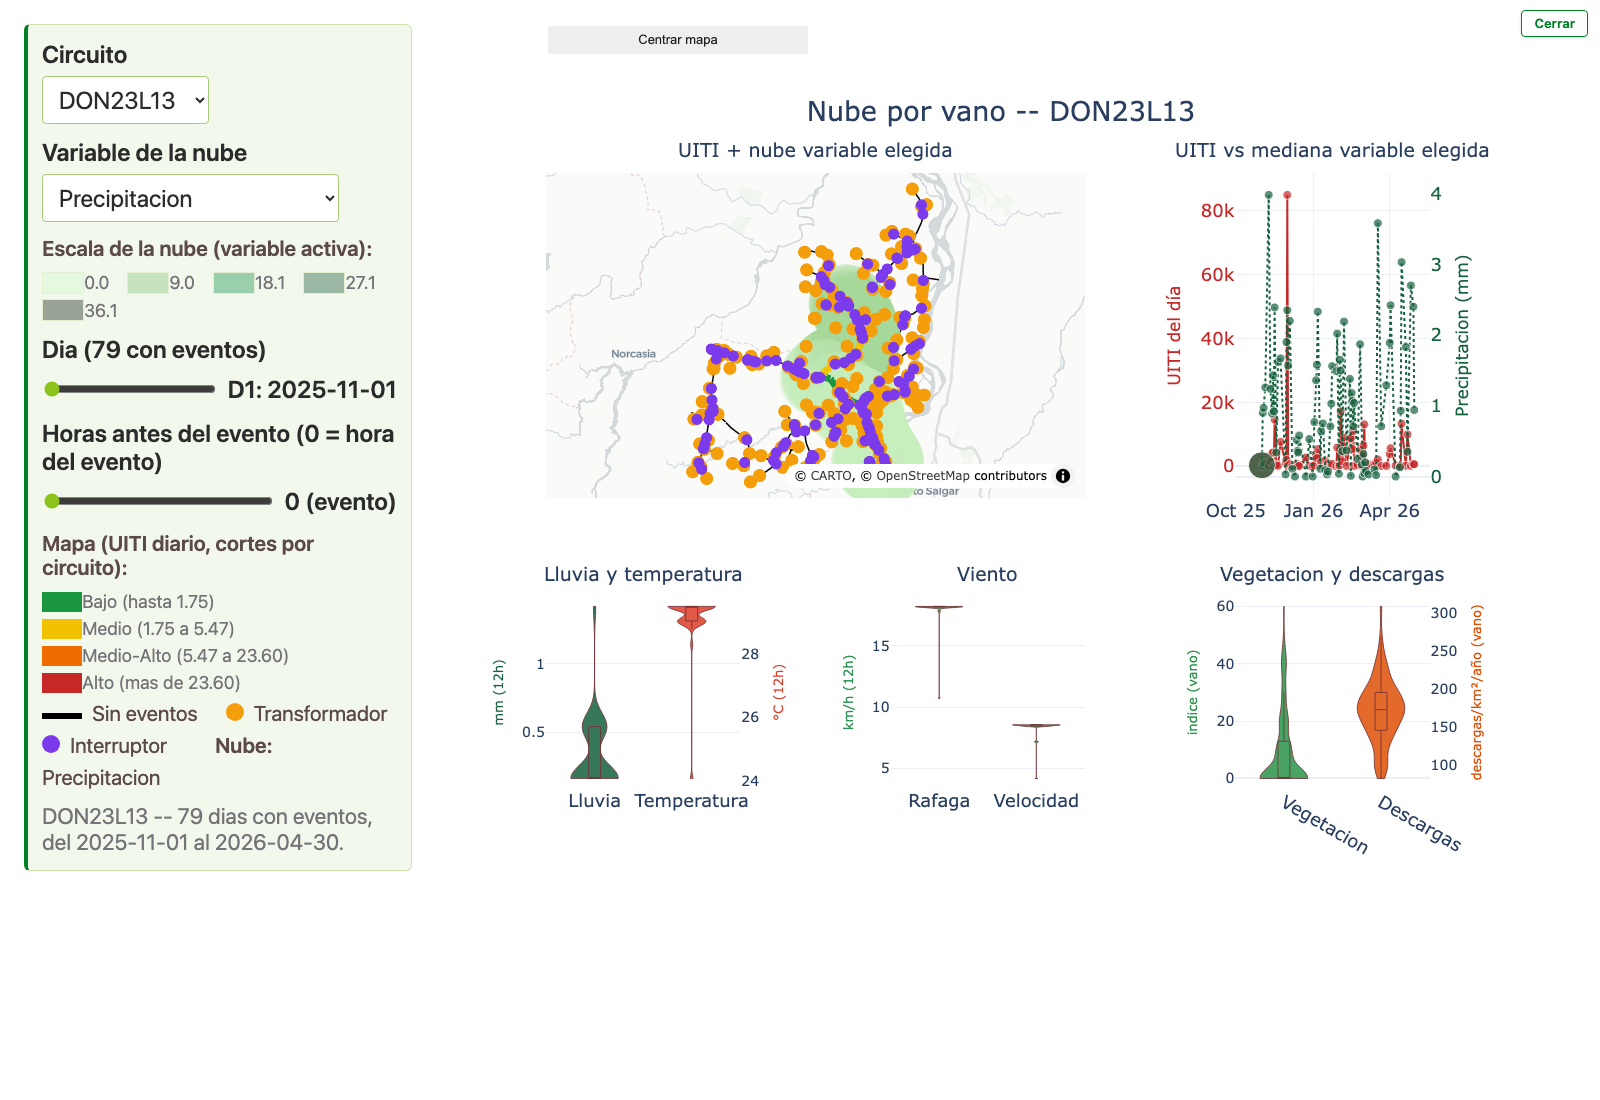
\includegraphics[width=0.94\textwidth]{figures/cuadernos/tablero_clima.png}
\caption{Nube por vano y clima del circuito DON23L13, con 79 días con eventos entre el 1 de
noviembre de 2025 y el 30 de abril de 2026. Sobre el mapa, la capa de \texttt{UITI\_VANO}
coloreada por umbrales y la nube de la variable climática del día seleccionado; a la derecha,
la serie de doble eje; abajo, los seis violines de distribución.}
\label{fig:clima}
\end{figure}

\subsubsection{Captura de datos climáticos con \texttt{/clima}}

Los datos climáticos se obtienen mediante el comando \texttt{/clima}, que consulta el servicio
Open-Meteo y ejecuta tres validaciones obligatorias antes de consumir cuota de la interfaz de
programación. La clave de la modalidad de pago la introduce el usuario en el momento,
permanece únicamente en memoria y no se almacena ni se registra en ninguna bitácora.

\begin{table}[H]
\centering
\caption{Compuertas de ejecución del comando \texttt{/clima}}
\label{tab:clima}
\footnotesize
\begin{tabularx}{\textwidth}{L{2.5cm} L{3.2cm} X}
\toprule
\textbf{Paso} & \textbf{Aspecto que resuelve} & \textbf{Detalle} \\
\midrule
Modo A o B & Destino de la salida &
El modo A reescribe \texttt{data/Indicadores\_vano\_v3.csv} con las coordenadas
\texttt{X1}/\texttt{Y1}. El modo B toma cualquier tabla de \texttt{data/} con
\texttt{XPOS1\_RED\_BASE}/\texttt{YPOS1\_RED\_AFECTA} y deja un archivo nuevo. \\
\addlinespace
Validación 1 & Ubicaciones &
Se ejecuta en primer lugar y es obligatoria: el proceso no continúa si no se dispone de
coordenadas válidas. \\
\addlinespace
Validación 2 & Modalidad gratuita o de pago &
La modalidad gratuita no requiere credenciales. La de pago solicita la clave al usuario en el
momento; no se persiste. \\
\addlinespace
Validación 3 & Límites de cuota &
Compara las llamadas necesarias contra el presupuesto disponible antes de iniciar la
descarga. Si la cuota es insuficiente, el proceso se detiene e informa la condición en lugar
de agotarla parcialmente. \\
\addlinespace
Salida & Ubicación del resultado &
Modo A: el mismo archivo v3. Modo B:
\texttt{data/clima\_<fuente>\_<inicio>\_a\_<fin>.csv}. El registro de consumo se escribe
aparte, en \texttt{.clima\_cache/}. \\
\addlinespace
Unificación & Concatenar ejecuciones &
Únicamente entre archivos con el mismo identificador de origen: combinar orígenes distintos
produciría una tabla estructuralmente válida y semánticamente inconsistente. \\
\bottomrule
\end{tabularx}
\end{table}

\subsection{Agrupamiento de vanos}

Este tablero cuantifica en qué vanos se concentra la criticidad de la red. Ajusta un
agrupamiento $K$-medias con $k=4$ sobre el par (UITI acumulado, número de eventos) de cada
vano, y nombra los grupos según el orden de la mediana del UITI --- nunca según el índice que
devuelve el algoritmo, que cambia entre ejecuciones.

El rango de fechas es ajustable y se redondea a meses completos; las etiquetas resultantes se
descargan a una hoja de cálculo. Sobre la ventana de referencia, el reparto es de 4.189 vanos
en Bajo ($15{,}3$\,\%), 11.449 en Medio ($41{,}8$\,\%), 10.314 en Medio-Alto ($37{,}7$\,\%) y
1.438 en Alto ($5{,}3$\,\%).

\begin{figure}[H]
\centering
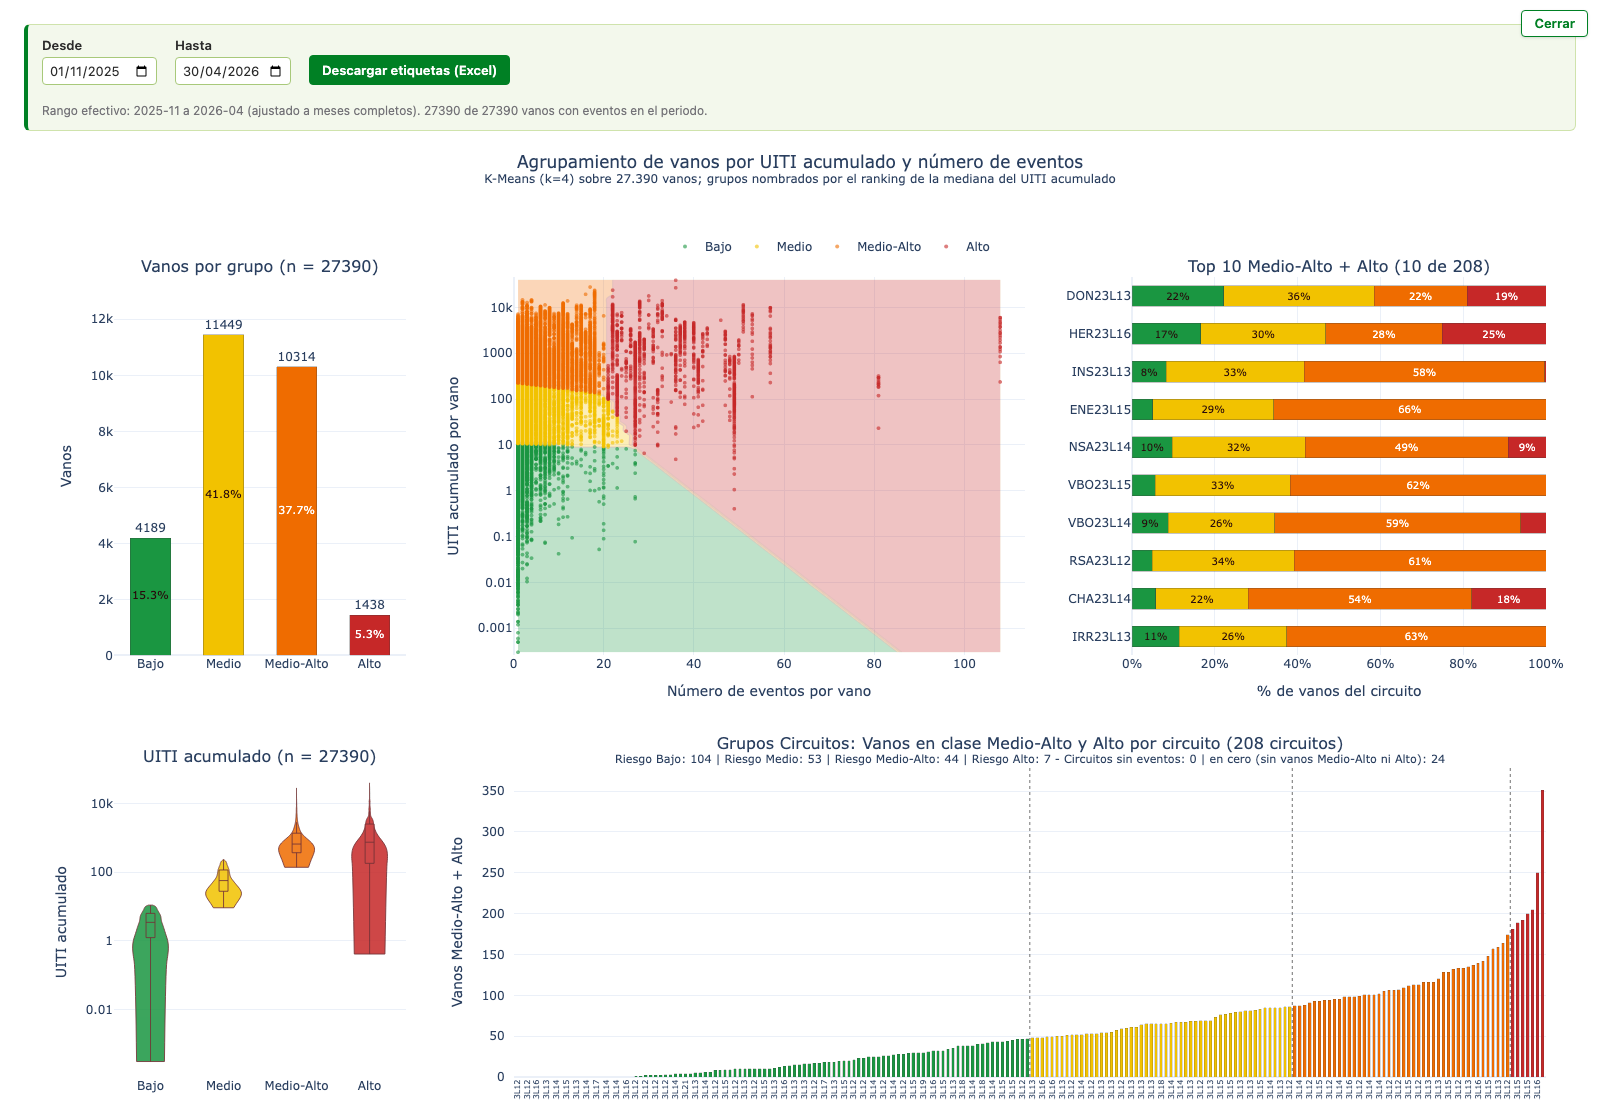
\includegraphics[width=0.94\textwidth]{figures/cuadernos/tablero_agrupamiento.png}
\caption{Agrupamiento de vanos por criticidad: 27.390 vanos con eventos entre noviembre de
2025 y abril de 2026, agrupados mediante $K$-medias con $k=4$ sobre el plano UITI acumulado
contra número de eventos.}
\label{fig:agrupamiento}
\end{figure}

\subsection{Trayectorias de circuitos}

Este tablero establece si un circuito mejora, se deteriora o se mantiene a lo largo del
periodo, y en qué ventana ocurre el cambio. Cada punto de la dispersión es un par
circuito $\times$ ventana, no un circuito: el mismo circuito aparece tantas veces como
ventanas registre, lo que permite observar su desplazamiento en el tiempo.

\begin{itemize}
  \item Ventana deslizante sobre las once ventanas del periodo, con sus fechas exactas a la
        vista.
  \item Mapa del circuito con el UITI del vano en la ventana activa, con los mismos cortes
        fijos.
  \item Trayectoria del circuito coloreada por el grupo de cada momento, que hace visible
        cuándo salta de grupo y cuándo retorna.
  \item Muestras, UITI y eventos por grupo, para leer la trayectoria contra la población
        completa.
\end{itemize}

\begin{figure}[H]
\centering
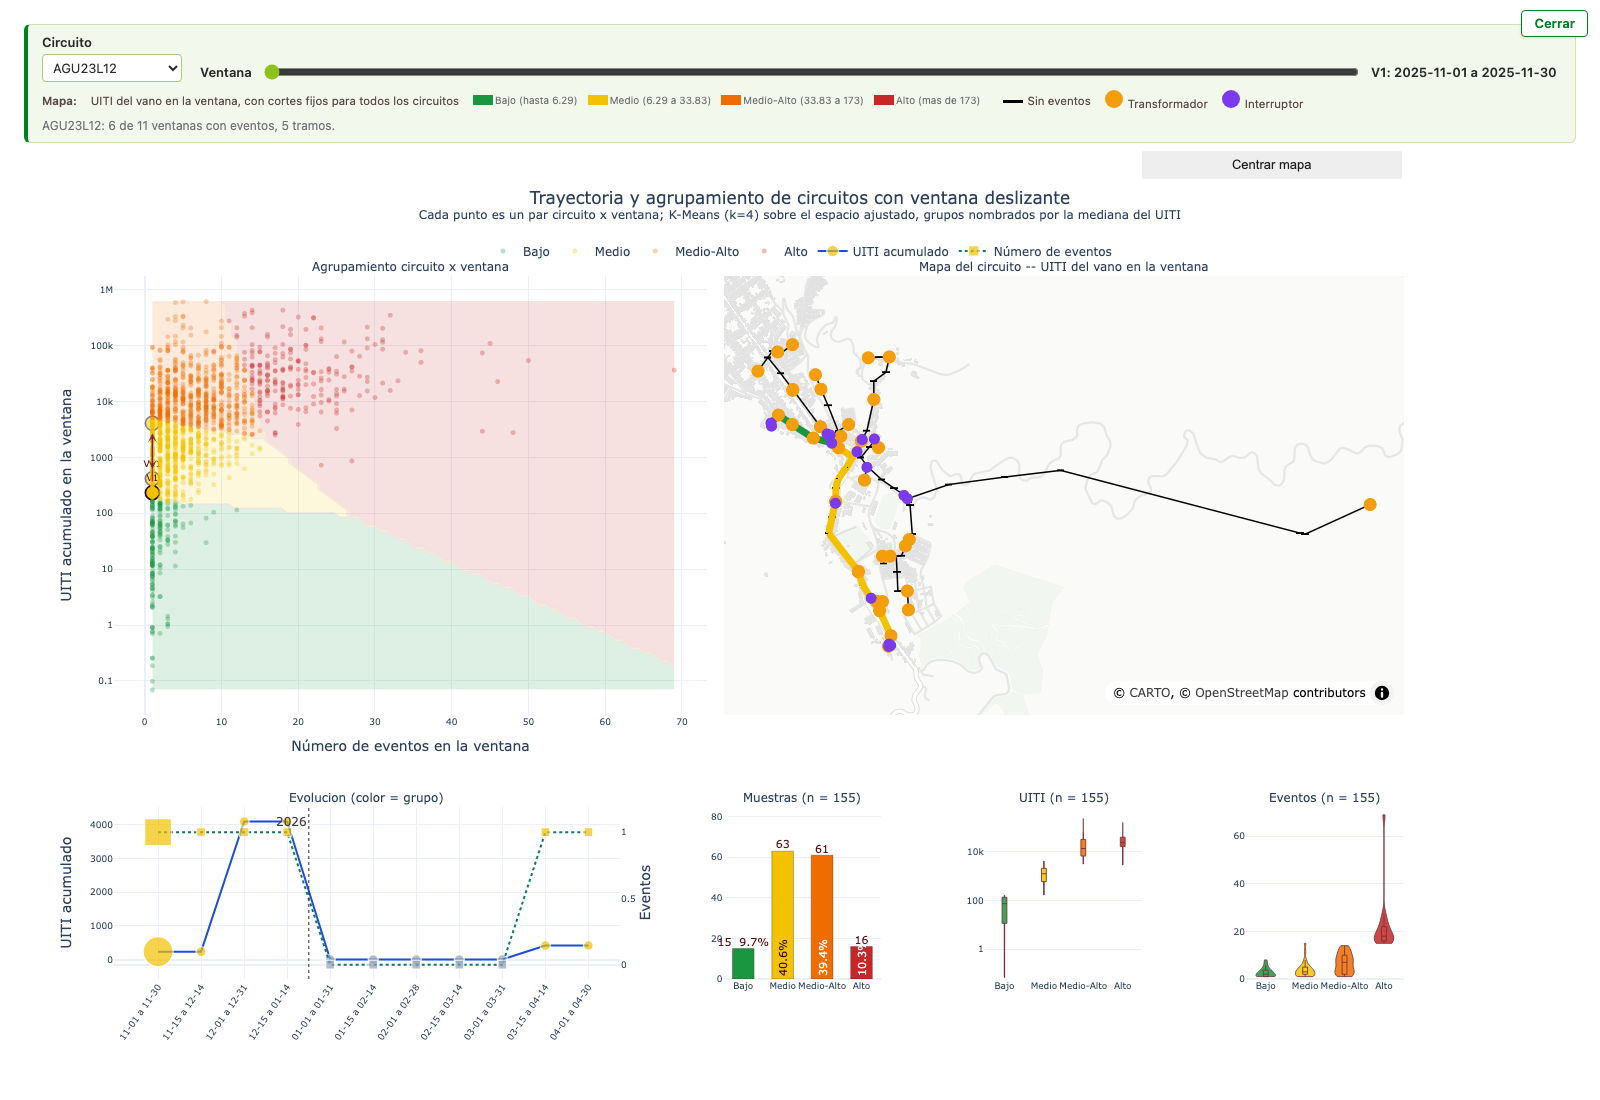
\includegraphics[width=0.94\textwidth]{figures/cuadernos/tablero_tray_circuitos.png}
\caption{Trayectorias del circuito AGU23L12, con 6 de sus 11 ventanas con eventos. La
dispersión sitúa cada par circuito $\times$ ventana sobre las cuatro regiones de criticidad;
el mapa georreferencia el circuito en la ventana activa.}
\label{fig:traycircuitos}
\end{figure}

\subsection{Trayectorias de vanos}

Este tablero traslada el análisis anterior a la unidad de intervención: la evolución de cada
vano ventana a ventana. El agrupamiento $K$-medias se ajusta una sola vez sobre la totalidad
de las celdas, de modo que los cortes no se recalculan al cambiar de circuito y dos circuitos
resultan comparables.

\begin{itemize}
  \item Selección de vanos mediante casillas, con acciones de marcar y desmarcar en bloque;
        la selección se aplica de forma simultánea a todos los paneles.
  \item Perfil del circuito, que informa cuánto del UITI del periodo concentran los vanos
        marcados. En el ejemplo de la Figura~\ref{fig:trayvanos}, 15 de 47 vanos explican el
        $88{,}3$\,\%.
  \item Evolución por vano, con UITI y número de eventos superpuestos ventana a ventana.
\end{itemize}

Este tablero no es únicamente un visor: la geometría de agrupamiento que produce es la que
consume después el cálculo de criticidad del modelo y del simulador, y los tres flujos que
dependen de ella la reutilizan en modo de solo lectura y verifican su firma antes de usarla.

\begin{figure}[H]
\centering
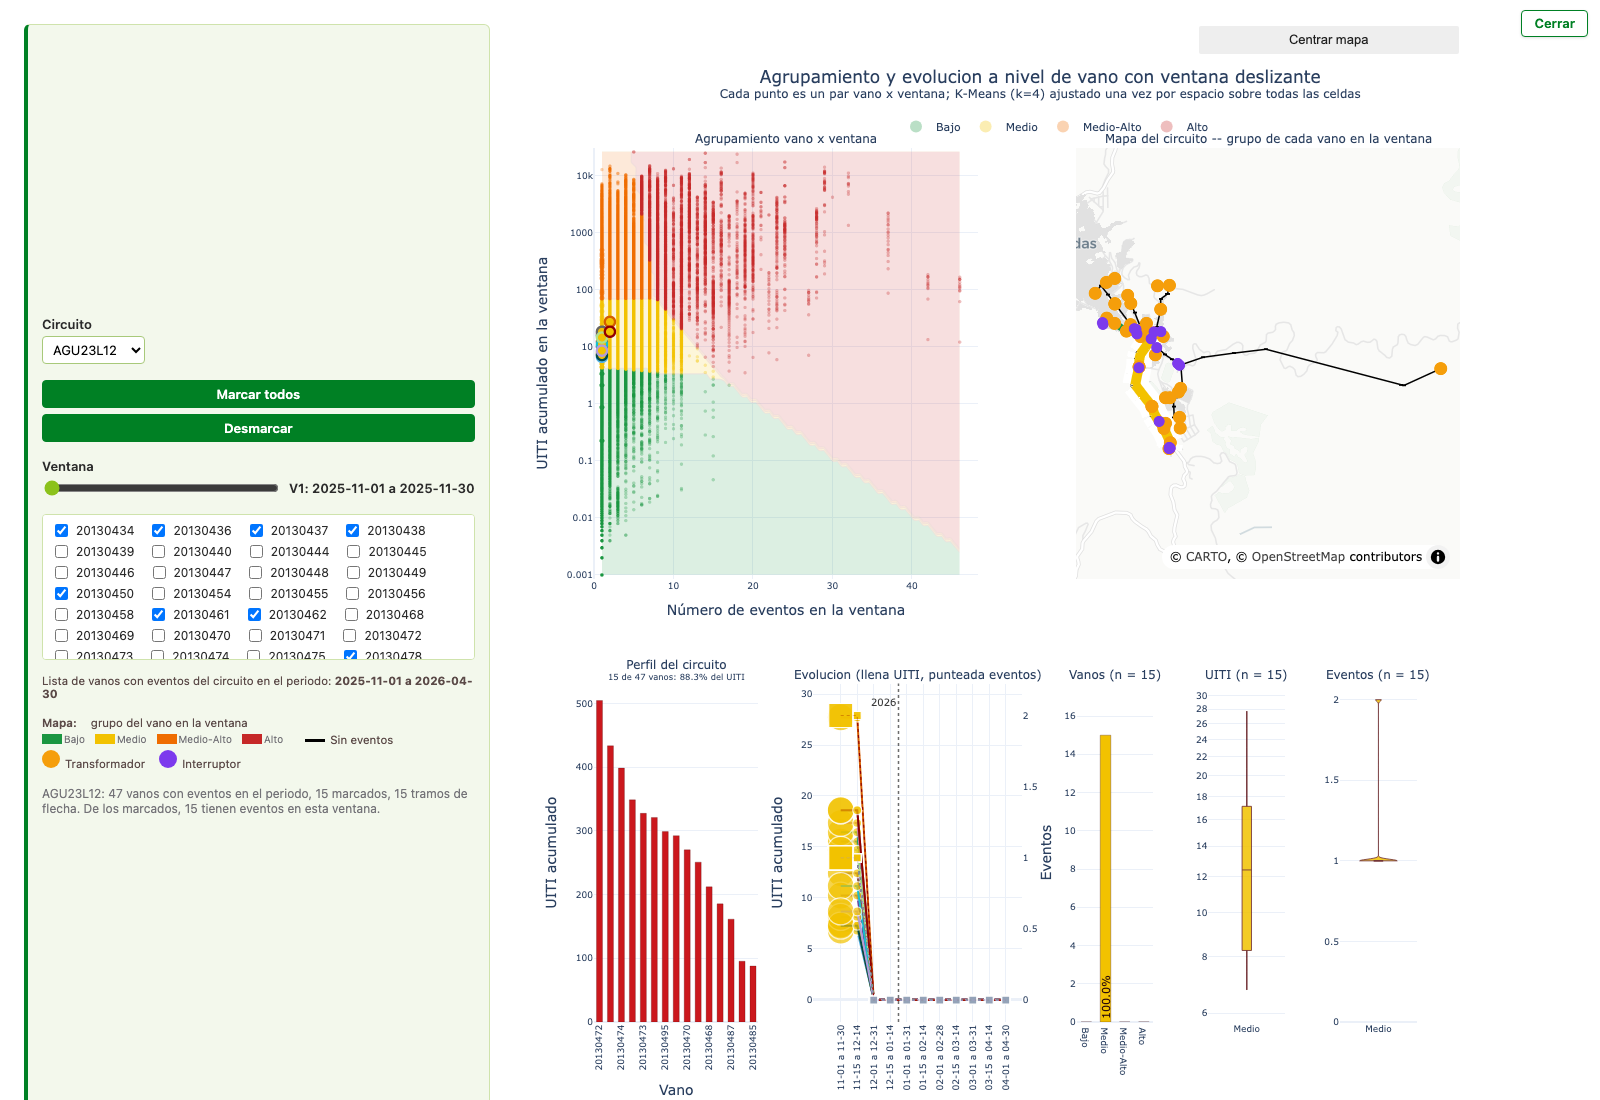
\includegraphics[width=0.94\textwidth]{figures/cuadernos/tablero_tray_vanos.png}
\caption{Trayectorias de vanos del circuito AGU23L12, con 15 de 47 vanos seleccionados que
concentran el $88{,}3$\,\% del UITI. Se presentan el panel de selección, el perfil del
circuito y la evolución por vano.}
\label{fig:trayvanos}
\end{figure}

\subsection{Del vano al grupo de circuito}
\label{sec:bandas}

La etiqueta de criticidad de un circuito no procede de un umbral definido manualmente. Se
obtiene en cuatro pasos encadenados, y la Figura~\ref{fig:cadena} los resume.

\begin{figure}[H]
\centering
\begin{tikzpicture}[node distance=8mm and 12mm]
  \node[blkg] (p1) {\textbf{1 $\cdot$ Celda vano $\times$ ventana}\\ 27.390 vanos con eventos\\ UITI acumulado y número de eventos};
  \node[blkd, right=of p1] (p2) {\textbf{2 $\cdot$ $K$-medias, $k=4$}\\ sobre ese plano de dos ejes;\\ devuelve 4 etiquetas sin orden propio};
  \node[blko, below=of p1] (p3) {\textbf{3 $\cdot$ Nombrado por mediana}\\ los 4 grupos se ordenan por la\\ mediana de su UITI acumulado\\ Bajo $\cdot$ Medio $\cdot$ Medio-Alto $\cdot$ Alto};
  \node[blk, below=of p2] (p4) {\textbf{4 $\cdot$ Ranking de circuitos}\\ 208 circuitos ordenados por\\ vanos Medio-Alto $+$ Alto\\ insumo del modelo predictivo};
  \draw[fl] (p1) -- (p2);
  \draw[fl] (p2) -- (p4);
  \draw[fl] (p4) -- (p3);
\end{tikzpicture}
\caption{Cadena que convierte el comportamiento observado de un vano en la banda de riesgo de
su circuito. El paso 3 corrige la arbitrariedad del índice que devuelve $K$-medias; el paso 4
sustituye el promedio por un conteo.}
\label{fig:cadena}
\end{figure}

Dos criterios explícitos sostienen esa cadena:

\begin{itemize}
  \item \textbf{Nombrado por mediana.} El algoritmo $K$-medias numera sus grupos con un orden
        que cambia entre ejecuciones. El nombre se asigna posteriormente a partir de la
        mediana del UITI, que sí constituye un criterio estable.
  \item \textbf{Conteo en lugar de promedio.} El promedio diluye el efecto de un número
        reducido de vanos críticos en circuitos con gran cantidad de vanos de baja
        criticidad. La clasificación contabiliza cuántos vanos caen en Medio-Alto y Alto, que
        es la carga efectiva.
\end{itemize}

\begin{figure}[H]
\centering
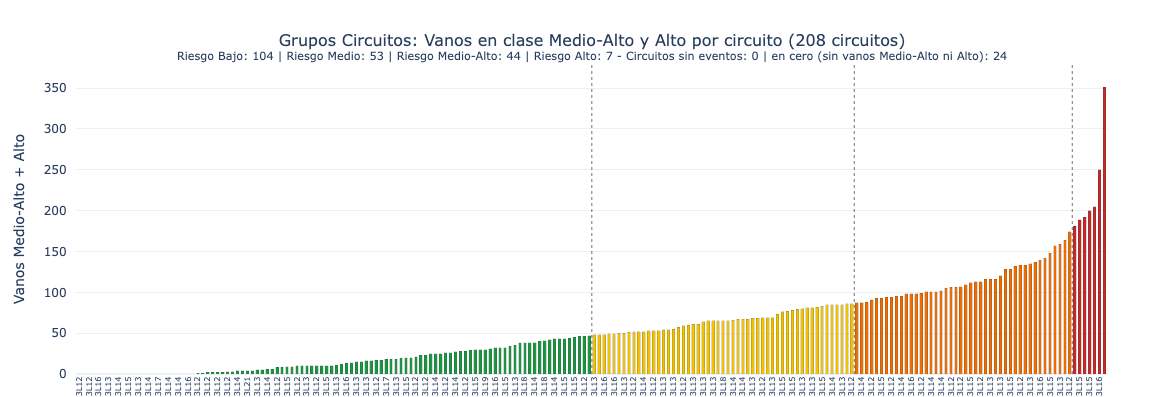
\includegraphics[width=0.92\textwidth]{figures/cuadernos/ranking_circuitos.png}
\caption{Clasificación de los 208 circuitos por número de vanos Medio-Alto y Alto, con los
cortes de las cuatro bandas de riesgo. Las etiquetas del eje horizontal son códigos de
circuito y a esta escala operan como referencia de densidad; el valor individual se consulta
en el tablero interactivo.}
\label{fig:ranking}
\end{figure}

\begin{table}[H]
\centering
\caption{Reparto de los 208 circuitos por banda de riesgo}
\label{tab:bandas}
\small
\begin{tabularx}{\textwidth}{L{4.2cm} c X}
\toprule
\textbf{Banda} & \textbf{Circuitos} & \textbf{Criterio} \\
\midrule
Bajo & 104 & Menor número de vanos en clase Medio-Alto y Alto. \\
Medio & 53 & \\
Medio-Alto & 44 & \\
Alto & 7 & Mayor concentración de vanos críticos. \\
\addlinespace
Sin vanos críticos & 24 & Circuitos sin ningún vano en Medio-Alto ni en Alto. \\
\bottomrule
\end{tabularx}
\end{table}

\paragraph{Un solo vocabulario de grupo.} Durante el desarrollo se identificaron dos criterios
para definir el grupo de un circuito: el resultado directo de $K$-medias sobre los circuitos y
la clasificación por número de vanos críticos. Para la categoría de riesgo alto, ambos
criterios coincidían únicamente en tres circuitos. Se adoptó como criterio definitivo la
clasificación por número de vanos Medio-Alto y Alto, y el primero se retiró del código, de
modo que un mismo nombre no designe dos particiones distintas.

\paragraph{Las ventanas se traslapan.} Cada vano aparece una vez por ventana, lo que convierte
el agrupamiento estático en una trayectoria temporal. Las once ventanas de treinta días se
solapan por construcción --- mes calendario más la ventana cruzada del 15 al 15 ---, de modo
que \textbf{el UITI no se suma entre ellas}: hacerlo contabilizaría varias veces el mismo
evento.

% ============================================== 7. MODELO =================
\section{Modelo de inteligencia artificial predictiva M-GCECDL}
\label{sec:modelo}

El módulo predictivo se denomina M-GCECDL, por \emph{Multimodal-Graph Connectivity Enhanced
and Conditioned Deep Learning}: un modelo de estimación de criticidad regularizado por
restricciones físicas y por un autocodificador del vector de características, construido desde
el análisis temporal de eventos sobre vanos mediante una representación por bolsas y múltiples
instancias.

\subsection{Unidad de análisis: la bolsa vano $\times$ ventana}

El modelo no puntúa un vano ni un evento: puntúa una \textbf{bolsa}. Una bolsa corresponde a un
par vano $\times$ ventana y contiene todas las instancias observadas de ese vano en esa
ventana. El enfoque es de aprendizaje por instancias múltiples: la etiqueta existe a nivel de
bolsa --- el UITI acumulado y su grupo de criticidad ---, mientras que las variables se
observan a nivel de instancia.

El preprocesamiento separa \texttt{UITI\_VANO} como objetivo del cual se derivan las clases, lo
que impide su uso como predictor. Las clases son cuatro niveles ordinales --- Bajo, Medio,
Medio-Alto y Alto --- obtenidos por vecino más cercano sobre la geometría de agrupamiento
$K$-medias descrita en la Sección~\ref{sec:bandas}, en el plano $(n_{\text{obs}}, u)$, donde
$n_{\text{obs}}$ es el número de eventos observados y $u$ el UITI acumulado. Esa geometría se
calcula una sola vez, se congela y se verifica por firma criptográfica: cualquier modificación
de los centroides interrumpe la ejecución con un error explícito, en lugar de desplazar las
clases derivadas sin registro.

El artefacto entrenado es un único archivo, \texttt{data/models/mil\_vano\_ventana\_v1.pt} de
691~KB, que transporta los pesos, los nombres de las 80 variables, la partición en
modalidades, el grafo de restricciones físicas proyectado, la geometría de agrupamiento y el
desglose de desempeño por clase. Esa autocontención permite que el visor del cuaderno, el
simulador y las aplicaciones lean el mismo modelo sin reconstruir nada.

\subsection{Arquitectura del modelo}

El modelo predice un escalar por bolsa, $\hat{p}_b \approx \log(1 + u_b)$, y deriva la clase con
la regla de vecino más cercano. La Figura~\ref{fig:modelo} presenta su diagrama de bloques.

\begin{figure}[H]
\centering
\begin{tikzpicture}[node distance=4.2mm and 6mm]

  \node[blk] (x) {$x_{\text{inst}}$ $(n_{\text{inst}} \times 80)$\\ $+$ índice de bolsa (CSR)};

  \node[blkd, below=12mm of x] (e1) {codificadores por modalidad\\ estructural (30) $\mid$ climática (50)};
  \node[blkd, below=of e1] (z1) {$z_1$ $(n_{\text{inst}} \times 128)$};
  \node[blkd, below=of z1] (ap) {atención por segmento\\ invariante a cardinalidad};
  \node[blkd, below=of ap] (zb) {$z_b$ $(n_{\text{bags}} \times 128)$};
  \node[blkd, below=of zb] (gd) {decodificador de compuertas\\ $g = 2\,\sigma(W z_b)$};
  \begin{scope}[on background layer]
    \node[grp, fit=(e1)(z1)(ap)(zb)(gd), label={[font=\scriptsize\bfseries,anchor=south west,yshift=1pt,fill=white,inner sep=1.5pt]north west:Paso 1 --- fuente de la compuerta}] (p1) {};
  \end{scope}

  \node[blkg, below=9mm of gd] (prop) {propagación sobre el grafo de restricciones \textbf{fijo}\\ $x' = x + \alpha\, g \odot A^{\top} x$, \; $\alpha = 0{,}2$};

  \node[blk, below=8mm of prop] (e2) {codificadores $+$ decodificadores\\ (los \emph{mismos} pesos)};
  \node[blk, below=of e2, xshift=-24mm] (rec) {características reconstruidas};
  \node[blk, below=of e2, xshift=14mm] (z2) {$z_2$ $(n_{\text{inst}} \times 128)$};
  \node[blk, below=of z2] (ap2) {la \emph{misma} atención\\ (pesos compartidos)};
  \node[blk, below=of ap2] (zb2) {$z_b^{(2)}$ $(n_{\text{bags}} \times 128)$};
  \begin{scope}[on background layer]
    \node[grp, fit=(e2)(rec)(z2)(ap2)(zb2), label={[font=\scriptsize\bfseries,anchor=south west,yshift=1pt,fill=white,inner sep=1.5pt]north west:Paso 2 --- el mismo módulo base}] (p2) {};
  \end{scope}

  \node[blko, below=9mm of zb2] (fus) {fusión FiLM: el clima modula lo estructural\\ $z^{\text{film}}_b = z^{\text{est}}_b \odot (1 + \gamma(z^{\text{clim}}_b)) + \beta(z^{\text{clim}}_b)$};
  \node[blko, below=of fus] (p) {$\hat{p}_b = \mathrm{cabeza}(z^{\text{film}}_b)$};
  \node[blko, below=of p] (cls) {\texttt{asignar\_clase}$\big(n_{\text{obs}}$ \textbf{observado}, $\mathrm{expm1}(\hat{p}_b)$, geometría$\big)$\\ $\rightarrow$ Bajo $\mid$ Medio $\mid$ Medio-Alto $\mid$ Alto};

  \draw[fl] (x) -- (e1);
  \draw[fl] (e1) -- (z1);
  \draw[fl] (z1) -- (ap);
  \draw[fl] (ap) -- (zb);
  \draw[fl] (zb) -- (gd);
  \draw[fl] (gd) -- (prop);
  \draw[fl] (x.east) -- ++(3.7,0) |- (prop.east);
  \draw[fl] (prop) -- (e2);
  \draw[fl] (e2) -- (rec);
  \draw[fl] (e2) -- (z2);
  \draw[fl] (z2) -- (ap2);
  \draw[fl] (ap2) -- (zb2);
  \draw[fl] (zb2) -- (fus);
  \draw[fl] (fus) -- (p);
  \draw[fl] (p) -- (cls);

\end{tikzpicture}
\caption{Diagrama de bloques del modelo por bolsas. La primera pasada produce la compuerta por
bolsa que modula el grafo de restricciones fijo; la segunda recodifica la entrada ya propagada
reutilizando exactamente los mismos pesos. La clase no procede de la red, sino de caer sobre la
geometría de agrupamiento congelada.}
\label{fig:modelo}
\end{figure}

El diseño garantiza tres propiedades con consecuencias directas sobre la validez de la
clasificación:

\begin{itemize}
  \item \textbf{Invarianza de cardinalidad.} Duplicar todas las instancias de una bolsa deja
        $\hat{p}_b$ idéntico. En ausencia de esta garantía el modelo podría acceder al número
        de eventos por una vía indirecta, siendo esa cantidad una de las dos coordenadas que
        definen la clase.
  \item \textbf{$n_{\text{obs}}$ es observado, nunca predicho.} De las dos coordenadas que
        determinan la clase, el modelo solo aporta $u$.
  \item \textbf{El grafo es fijo.} Se registra como memoria intermedia y no como parámetro, de
        modo que ninguna arista se aprende. El único elemento ajustable en todo el camino del
        grafo es la compuerta $g_b$, que escala por bolsa las aristas existentes sin crear ni
        eliminar ninguna.
\end{itemize}

\subsection{Variables de entrada}

El modelo opera sobre una matriz de 80 columnas por instancia, repartidas en dos modalidades:
30 estructurales --- vano, transformador, topología y las diez columnas derivadas de
\texttt{COD\_CAUSA}, es decir su frecuencia relativa y nueve indicadores --- y 50 climáticas
--- riesgo por vegetación, descargas a tierra y cuatro series meteorológicas con doce rezagos
cada una.

\begin{table}[H]
\centering
\caption{Familias de variable que ingresan al modelo}
\label{tab:variables}
\footnotesize
\begin{tabularx}{\textwidth}{L{3.2cm} L{3.4cm} X}
\toprule
\textbf{Familia} & \textbf{Tipo} & \textbf{Ejemplos} \\
\midrule
Estructural del vano & Numérica & \texttt{ALTURA}, \texttt{CNT\_FASES}, \texttt{LONG\_CRUCETA}, \texttt{VAL\_CRIT\_APOYO}, \texttt{CANTIDAD\_TIERRA} \\
Estructural del vano & Categórica & \texttt{CONDUCTOR}, \texttt{TIPO}, \texttt{CALIBRE\_NEUTRO}, \texttt{NG\_RED}, \texttt{TIPO\_TAX} \\
Transformador & Numérica & \texttt{CAPACIDAD\_NOMINAL}, \texttt{PROMEDIO\_KWH\_TRF}, \texttt{CNT\_TRF} \\
Topología & Numérica & \texttt{CNT\_VN}: vanos hasta el equipo que protege el tramo \\
Entorno & Numérica & \texttt{NR\_T}: riesgo por vegetación \\
Clima & Serie con 12 rezagos & Precipitación, temperatura, viento, ráfaga y descargas a tierra \\
Evento & Categórica codificada & \texttt{COD\_CAUSA}, su frecuencia relativa y nueve indicadores \\
Espacio y tiempo & Coordenada y fecha & \texttt{X2}, \texttt{Y2}, \texttt{FECHA\_OPERACION\_VANO} \\
Objetivo & Numérica por bolsa & \texttt{UITI\_VANO} acumulado en la ventana \\
\bottomrule
\end{tabularx}
\end{table}

\subsection{Formulación matemática}

\paragraph{Agregación de la bolsa.} La atención opera por segmento, es decir una distribución
por bolsa y no por lote:

\begin{equation}
e_i = w^{\top}\tanh(V z_i), \qquad
a_i = \frac{\exp(e_i)}{\sum_{j \in b(i)} \exp(e_j)}, \qquad
z_b = \sum_{i \in b} a_i\, z_i .
\end{equation}

\paragraph{Propagación por el grafo.} La compuerta por bolsa
$g_b = 2\,\sigma(W z_b) \in (0,2)^{E}$ modula el grafo fijo y escribe únicamente en las
columnas destino de las $E$ aristas:

\begin{equation}
x'_i = x_i + \alpha \sum_{(r \to c)\, \in\, \mathcal{E}} g_{b(i),\,rc}\; A_{rc}\; x_{i,r}\; \mathbf{e}_c .
\end{equation}

\paragraph{Función de costo.} Sobre un lote de $B$ bolsas, con $t_b = \log(1 + u_b)$ el
objetivo de la bolsa $b$, la pérdida activa reúne cuatro términos:

\begin{equation}
\mathcal{L}
= \lambda_{\mathrm{sup}}\mathcal{L}_{\mathrm{sup}}
+ \lambda_{\mathrm{rec}}\tilde{\mathcal{L}}_{\mathrm{rec}}
+ \lambda_{\mathrm{MI}}\mathcal{L}_{\mathrm{MI}}
+ \lambda_{\mathrm{cl}}\mathcal{L}_{\mathrm{cl}} .
\label{eq:costo}
\end{equation}

El término supervisado es un error cuadrático ponderado por la densidad inversa del objetivo,
lo que evita que la cola alta de UITI quede dominada por la masa central de la distribución:

\begin{equation}
\mathcal{L}_{\mathrm{sup}} = \frac{1}{B}\sum_{b} \tilde{w}(t_b)\,(\hat{p}_b - t_b)^2,
\qquad
w(t) = \frac{1}{\max\!\big(\hat{f}_{\mathrm{KDE}}(t),\,\varepsilon\big)},
\qquad
\tilde{w} = \frac{w}{\bar{w}} .
\end{equation}

La densidad $\hat{f}_{\mathrm{KDE}}$ se ajusta una sola vez sobre el pliegue de entrenamiento
--- higiene de pliegue --- y los pesos se renormalizan a media unitaria por lote, de manera que
la escala resulte comparable con un error cuadrático plano.

El término de reconstrucción se calcula contra la entrada estandarizada $z=(x-\mu)/\sigma$ y se
acota sin anular el gradiente:

\begin{equation}
\mathcal{L}^{\mathrm{raw}}_{\mathrm{rec}} = \frac{1}{n p}\sum_{i,j}(\hat{x}_{ij} - z_{ij})^2,
\qquad
\tilde{\mathcal{L}}_{\mathrm{rec}} = \frac{\mathcal{L}^{\mathrm{raw}}_{\mathrm{rec}}}{1 + \mathcal{L}^{\mathrm{raw}}_{\mathrm{rec}}} \in [0,1) .
\end{equation}

Su objetivo es el $x$ original y no $x'$. De emplearse $x'$, la compuerta --- único elemento
ajustable del camino del grafo --- controlaría su propio objetivo y podría reducir la pérdida
simplificándolo, sin mejorar la representación.

El término de información mutua es el único que ata la representación aprendida a la estructura
declarada. Compara, mediante información mutua cuadrática de Rényi, un núcleo gaussiano sobre
los perfiles de variables reconstruidas contra el núcleo del grafo fijo:

\begin{equation}
\mathcal{L}_{\mathrm{MI}} = 1 - \bar{I}_2(K_r, K_g),
\qquad
\bar{I}_2 = \frac{I_2}{\log p} .
\end{equation}

$K_g$ no se estima de los datos: se construye una sola vez en el constructor de la pérdida a
partir de la lista de nombres de las variables, se almacena como constante y no recibe
gradiente. El lado declarado es invariante por construcción, de modo que el término solo puede
aproximar la representación aprendida a la estructura del grafo, y no el grafo a los datos.

Finalmente, el término de clase es una entropía cruzada sobre las fronteras de la geometría
congelada, diferenciable a través de $\hat{p}_b$:

\begin{equation}
\hat{u}_b = \mathrm{softplus}\!\big(\mathrm{expm1}(\hat{p}_b)\big),
\qquad
\mathcal{L}_{\mathrm{cl}} = \mathrm{CE}\!\left(-\frac{d^2\big(n^{\mathrm{obs}}_b,\, \hat{u}_b\big)}{T},\; c^{*}_b\right),
\qquad T = 0{,}01 .
\end{equation}

Sin este término, ningún componente del costo incorporaría la posición de las fronteras entre
centroides, que es precisamente lo que evalúa la métrica de desempeño. La temperatura no hereda
el valor unitario de otros usos del proyecto: con distancias cuadradas de mediana $0{,}038$, una
temperatura unitaria deja la distribución \emph{softmax} prácticamente uniforme --- entropía de
$1{,}3850$ contra $\ln 4 = 1{,}3863$ --- y el término queda en su piso desde la primera época.
La clase objetivo $c^{*}_b$ se deriva de lo observado con la misma geometría y no se recibe por
parámetro, lo que impide introducir un objetivo inconsistente con la regla de asignación.

\begin{table}[H]
\centering
\caption{Pesos del artefacto entrenado y participación del grafo fijo en cada término}
\label{tab:terminos}
\small
\begin{tabularx}{\textwidth}{L{3.5cm} c L{2.4cm} X}
\toprule
\textbf{Término} & \textbf{Peso} & \textbf{Usa el grafo} & \textbf{Papel} \\
\midrule
Supervisado & $1{,}00$ & Indirecto & No aparece en la fórmula; entra porque $\hat{p}_b$ se calcula sobre $x'$. \\
Reconstrucción & $0{,}01$ & No & Deliberado: el objetivo es el $x$ original. \\
Información mutua & $0{,}01$ & Sí, como referencia & Único término que ata la representación a la estructura declarada. \\
Clase & $1{,}00$ & No & Usa la geometría de centroides, artefacto fijo distinto del grafo. \\
\addlinespace
Desviación de compuertas & $0{,}00$ & Sí, como ancla & Penalizaría apartarse del grafo tal como fue declarado. Desactivado. \\
Supervisión por modalidad & $0{,}00$ & No & Inerte bajo la fusión FiLM; solo resulta pertinente bajo fusión por confiabilidad. \\
\bottomrule
\end{tabularx}
\end{table}

Corresponde registrar una limitación de orden cuantitativo y no conceptual: los dos términos del
grafo están acotados en $[0,1]$ y pesan $0{,}01$ cada uno, por lo que su contribución conjunta
al costo total no supera $0{,}02$, frente a un término supervisado cuyo rango observado fue de
$0{,}35$ a $6{,}8$. Con esta configuración la participación del grafo en el gradiente es
marginal, y su aporte efectivo requiere una ablación explícita para ser establecido.

Los hiperparámetros del artefacto vigente son: dimensión oculta 128, dimensión de embebido 64,
dimensión de atención 64, \emph{dropout} $0{,}1$, $\alpha = 0{,}2$, tasa de aprendizaje
$10^{-3}$, decaimiento de pesos $10^{-5}$, lotes de 256 bolsas, 30 épocas y 5 pliegues, con
semilla fija.

\subsection{Grafo de restricciones físicas}
\label{sec:grafo}

Las relaciones entre variables no se aprenden de forma autónoma: se declaran previamente
mediante un grafo de restricciones físicas, definido en código por la función
\texttt{construir\_\allowbreak aristas\_\allowbreak grafo\_\allowbreak chec} y almacenado dentro del artefacto \texttt{.pt}. Esa
ubicación garantiza que el simulador, los informes y el cuaderno operen sobre exactamente la
misma estructura.

El grafo declarado comprende \textbf{156 relaciones dirigidas sobre 156 variables} y es
acíclico: todo camino avanza hacia \texttt{UITI\_VANO}, que es su único destino final. Sus
pesos son juicio experto declarado variable por variable --- valores como $0{,}60$, $0{,}75$ o
$0{,}90$ --- y no correlaciones estimadas de los datos. Lo único que los datos determinan es
qué nodos existen: si un código de causa no alcanza el umbral de frecuencia relativa del
$1$\,\%, su columna no está y las aristas que lo tocaban no se proyectan.

Su composición, verificada sobre el código vigente, es la siguiente:

\begin{table}[H]
\centering
\caption{Composición de las 156 relaciones declaradas del grafo}
\label{tab:grafocomposicion}
\small
\begin{tabularx}{\textwidth}{L{5.6cm} c X}
\toprule
\textbf{Clase de relación} & \textbf{Cantidad} & \textbf{Descripción} \\
\midrule
Cadena de rezago climático & 99 & Nueve familias meteorológicas $\times$ once enlaces entre rezagos consecutivos, con peso $0{,}90$. \\
Rezago cero hacia la causa & 9 & Cada familia en la hora del evento alimenta \texttt{COD\_CAUSA}, con peso $0{,}85$. \\
Ráfaga hacia riesgo vegetal & 1 & \texttt{wind\_gust\_spd\_0} $\rightarrow$ \texttt{NR\_T}, con peso $0{,}80$. \\
Relaciones de dominio & 47 & Recorren el camino desde la geometría del vano hasta el cálculo de \texttt{UITI\_VANO}. \\
\midrule
\textbf{Total declarado} & \textbf{156} & \\
\bottomrule
\end{tabularx}
\end{table}

La selección de variables elimina después una parte de esos nodos. En lugar de descartar las
aristas que tocaban un nodo eliminado, un recorrido en anchura busca, desde cada nodo
conservado, el primer nodo también conservado que sea alcanzable a través de los eliminados, y
registra una \emph{arista virtual} con el peso mínimo del trayecto. El mínimo es la elección
conservadora: una cadena no puede declararse más fuerte que su eslabón más débil. Sobre el
artefacto vigente el resultado es una matriz de adyacencia de $80 \times 80$ con
\textbf{64 aristas no nulas}.

\begin{sidewaysfigure}
\centering
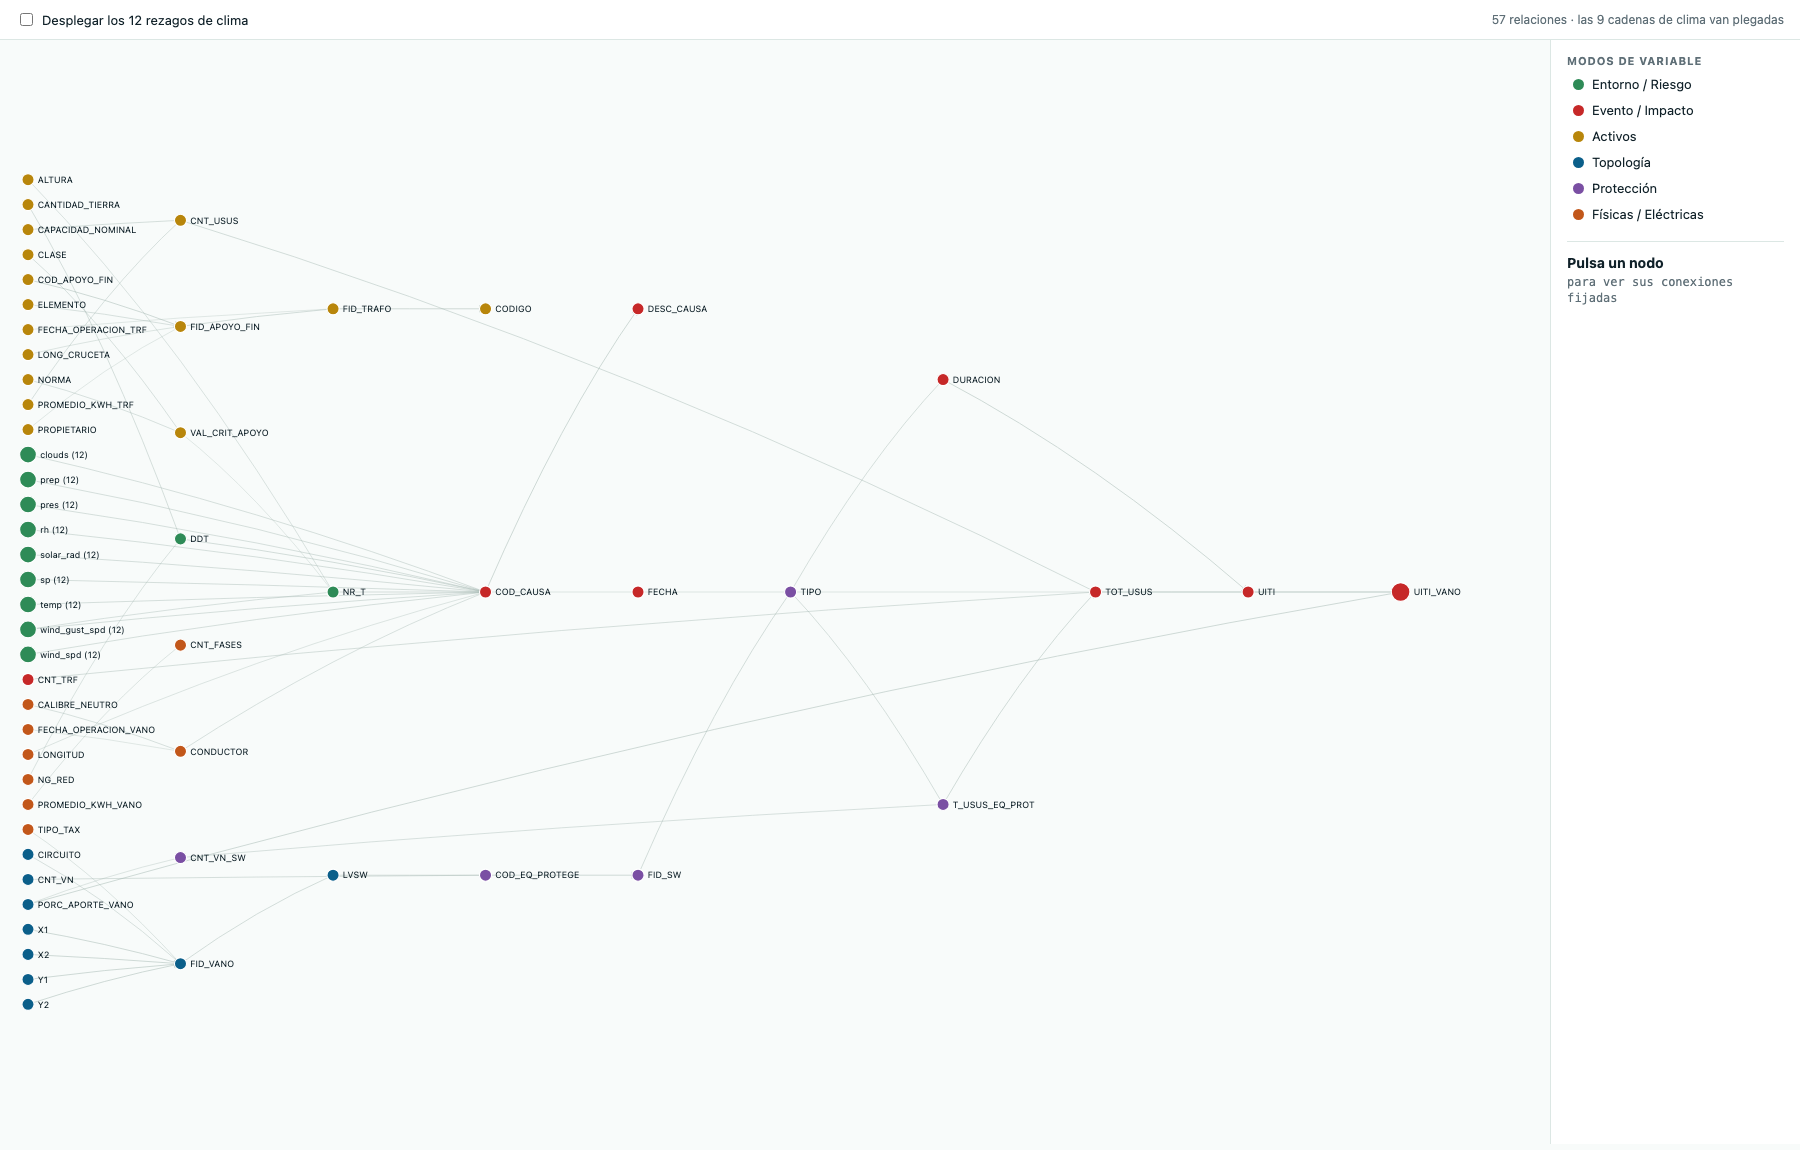
\includegraphics[width=0.95\textheight]{figures/informe/grafo_fijo_mil.png}
\caption{Grafo de restricciones físicas del modelo, con las nueve cadenas de rezago climático
plegadas: se representan 57 de las 156 relaciones declaradas. Los nodos se colorean por modo de
variable y \texttt{COD\_CAUSA} concentra el mayor grado de entrada. En el visor interactivo, al
seleccionar un nodo se despliegan sus relaciones de entrada, sus relaciones de salida y los
pesos asociados.}
\label{fig:grafofijo}
\end{sidewaysfigure}

\subsubsection{Alcance de cada modo dentro del grafo}

Las variables se agrupan en seis modos, y el grafo define qué relaciones se permiten entre
ellos. La tercera columna de la Tabla~\ref{tab:modos} no constituye interpretación libre:
recoge lo que el análisis de criticidad del proyecto declara que se busca en cada relación, y
es también el marco con el que los agentes leen el modelo.

\begin{table}[H]
\centering
\caption{Modos de variable, conexiones fijadas y relaciones evaluadas}
\label{tab:modos}
\footnotesize
\begin{tabularx}{\textwidth}{L{2.4cm} L{4.6cm} X}
\toprule
\textbf{Modo} & \textbf{Conexiones fijadas en el grafo} & \textbf{Relaciones y posibles causas evaluadas} \\
\midrule
Entorno / Riesgo &
Hacia el mismo modo (100) y hacia Evento / Impacto (11). &
Acumulación del estrés ambiental en las doce horas previas: cada rezago apunta al siguiente,
de modo que la cadena representa la condición antecedente y no el instante del evento. Es la
vía por la que el modelo puede sostener una hipótesis ambiental, nunca afirmarla. \\
\addlinespace
Físicas / Eléctricas &
Hacia el mismo modo (3), Evento / Impacto (2), Entorno / Riesgo (1) y Topología (1). &
Características constructivas que se explican entre sí y que modulan la susceptibilidad del
tramo: conductor, longitud y calibre del neutro. La ausencia de cable de guarda o neutro
incrementa la exposición a las descargas. \\
\addlinespace
Activos &
Hacia el mismo modo (11), Entorno / Riesgo (3) y Evento / Impacto (1). &
Encadenan apoyo, transformador y sus atributos para identificar el activo afectado, y
cuantifican la carga servida aguas abajo. Estas variables explican la magnitud del impacto, no
su frecuencia. \\
\addlinespace
Topología &
Hacia el mismo modo (6), Protección (3) y Evento / Impacto (1). &
Ubican el tramo y determinan el alcance del equipo que lo protege --- número de vanos que cubre
y distancia ---, lo que fija el alcance de una interrupción, y establecen la fracción del
impacto del circuito que corresponde al vano. \\
\addlinespace
Protección &
Hacia el mismo modo (4) y Evento / Impacto (2). &
Correspondencia entre vano y equipo de protección, y efecto del tipo de equipo sobre la
duración de la interrupción y el número de usuarios afectados aguas abajo. \\
\addlinespace
Evento / Impacto &
Hacia el mismo modo (7). &
Descomposición del UITI: duración por usuarios afectados y, a partir de ahí, el aporte del
vano. \\
\bottomrule
\end{tabularx}
\end{table}

El grafo restringe las relaciones que el modelo puede utilizar, pero \textbf{no establece
causalidad}. Una relación fijada indica que el modelo puede emplear esa relación, no que el
fenómeno ocurra: la vía de \texttt{NR\_T} hacia \texttt{COD\_CAUSA} existe para que la
vegetación pueda sostener una hipótesis de causa, y esa hipótesis requiere respaldo en los
datos observados dentro de la ventana analizada. Por esa razón los informes se expresan en
términos de lo que resulta compatible con la evidencia, y no de lo que la causó.

\subsection{Aplicación sobre datos nuevos}

El procedimiento de inferencia sobre observaciones que el modelo no vio durante el
entrenamiento consta de cinco pasos:

\begin{enumerate}
  \item Se arma la matriz de instancias con el mismo codificador de \texttt{COD\_CAUSA}
        empleado en el entrenamiento.
  \item Se carga el artefacto \texttt{.pt}, que aporta los pesos, el grafo de restricciones y
        la geometría de agrupamiento congelada.
  \item Cada fila ingresa como bolsa unitaria con $n_{\text{obs}} = 1$, que es lo correcto al
        evaluar eventos individuales.
  \item La red devuelve $\hat{u}$ y la función de asignación determina la clase a partir de la
        geometría.
  \item El mecanismo de atención proporciona, por bolsa, la contribución relativa de las
        variables de mayor peso, que constituye el insumo del diagnóstico del simulador.
\end{enumerate}

\subsection{Protocolo de validación y resultado}
\label{sec:validacion}

La métrica es macro-F1 fuera de pliegue, con validación cruzada estratificada y agrupada por la
clave $(\texttt{CIRCUITO}, \texttt{FID\_VANO})$, de modo que ninguna bolsa de un mismo vano
cruce la frontera entre pliegues. Las ventanas se solapan por construcción, así que sin ese
control un mismo evento aparecería a ambos lados de la partición. La evaluación se restringe al
subconjunto de bolsas cuyo vano tiene al menos dos ventanas y cuya clase observada no es
constante entre ellas: deliberadamente, el subconjunto difícil.

El modelo se contrasta contra tres líneas base: predicción mayoritaria, un bosque aleatorio
sobre las variables estructurales sin clima, y persistencia de la clase de la ventana anterior.

\begin{table}[H]
\centering
\caption{Desempeño fuera de pliegue del modelo y de sus tres líneas base, sobre 62.114 bolsas}
\label{tab:brazos}
\small
\begin{tabularx}{\textwidth}{X r r}
\toprule
\textbf{Brazo} & \textbf{Exactitud} & \textbf{macro-F1} \\
\midrule
Bosque aleatorio estructural (mejor línea base) & $0{,}8653$ & $0{,}8812$ \\
Modelo M-GCECDL & $0{,}8535$ & $0{,}8710$ \\
Persistencia & $0{,}4484$ & $0{,}3821$ \\
Mayoritaria & $0{,}4384$ & $0{,}1524$ \\
\bottomrule
\end{tabularx}
\end{table}

\begin{table}[H]
\centering
\caption{Desempeño del modelo por grupo de criticidad}
\label{tab:porclase}
\small
\begin{tabularx}{\textwidth}{X r r r r}
\toprule
\textbf{Grupo} & \textbf{Precisión} & \textbf{Exhaustividad} & \textbf{F1} & \textbf{Soporte} \\
\midrule
Bajo       & $0{,}8443$ & $0{,}8252$ & $0{,}8346$ & 13.323 \\
Medio      & $0{,}8295$ & $0{,}8514$ & $0{,}8403$ & 27.229 \\
Medio-Alto & $0{,}8571$ & $0{,}8453$ & $0{,}8512$ & 15.220 \\
Alto       & $0{,}9741$ & $0{,}9421$ & $0{,}9578$ & \phantom{0}6.342 \\
\bottomrule
\end{tabularx}
\end{table}

\begin{table}[H]
\centering
\caption{Resultado del protocolo de validación con barra preregistrada}
\label{tab:validacion}
\small
\begin{tabularx}{\textwidth}{X r}
\toprule
\textbf{Concepto} & \textbf{Valor} \\
\midrule
Bolsas evaluadas en validación cruzada agrupada & 62.114 \\
macro-F1 del modelo & $0{,}8710$ \\
macro-F1 de la mejor línea base & $0{,}8812$ \\
Barra de aceptación preregistrada & $+5{,}0$ puntos \\
Diferencia observada & $-1{,}02$ puntos \\
\textbf{Veredicto} & \textbf{No alcanzado} \\
\bottomrule
\end{tabularx}
\end{table}

El resultado se reporta junto con los matices que un veredicto binario no recoge. Ninguna clase
queda sin predicciones; la clase Alto registra el mejor desempeño del modelo, con F1 de
$0{,}958$, y el error se concentra en clases contiguas --- la confusión entre Bajo y Alto ocurre
una vez en 13.323 casos ---, perfil adecuado para priorización operativa.

La consideración determinante es que \textbf{la brecha es menor que el ruido del propio
entrenamiento}. Dos corridas de configuración idéntica arrojaron $0{,}8012$ y $0{,}8710$, es
decir siete puntos de dispersión atribuibles al no determinismo de la ejecución, mientras que la
línea base reprodujo su valor de forma idéntica en seis corridas. Bajo esa dispersión, la
diferencia de $-1{,}02$ puntos no permite concluir sobre la calidad relativa de los modelos, y la
estabilización del determinismo del entrenamiento constituye un prerrequisito y no una mejora
opcional.

\subsection{Dónde se entrena}

El cuaderno resuelve el dispositivo de cómputo automáticamente, y esa elección resultó
equivocada al medirla. Sobre un pliegue real de 88.987 bolsas se cronometraron tres épocas y se
proyectó la validación cruzada completa.

\begin{table}[H]
\centering
\caption{Tiempo y memoria del entrenamiento por dispositivo, medidos en el equipo de referencia}
\label{tab:dispositivo}
\small
\begin{tabularx}{\textwidth}{X r r r}
\toprule
\textbf{Dispositivo} & \textbf{s / época} & \textbf{Proyección completa} & \textbf{Pico de memoria} \\
\midrule
CPU, 2 hilos  & $3{,}28$  & $8{,}2$ min  & 3.293 MB \\
CPU, 4 hilos  & $3{,}61$  & $9{,}0$ min  & 3.288 MB \\
CPU, 8 hilos  & $4{,}60$  & $11{,}5$ min & 3.275 MB \\
CPU, 14 hilos & $5{,}51$  & $13{,}8$ min & 3.267 MB \\
GPU integrada (MPS) & $19{,}63$ & $49{,}1$ min & 11.234 MB \\
\bottomrule
\end{tabularx}
\end{table}

Dos lecturas se derivan de esa medición, y ninguna es la esperable. La GPU integrada del propio
procesador resulta seis veces más lenta y demanda $3{,}4$ veces más memoria que la CPU del mismo
equipo: el modelo, con 150.926 parámetros, es demasiado pequeño para amortizar el traslado de
cada lote. Y un mayor número de núcleos empeora el tiempo de forma monótona, porque coordinar
hilos cuesta más que el trabajo que reparten.

\textbf{Ninguna parte del proyecto requiere GPU.} Un equipo de dos o cuatro núcleos y 8~GB de
memoria reentrena este modelo en unos diez minutos. El pico de memoria lo fija la preparación de
datos --- leer el archivo de eventos cuesta $2{,}4$~GB --- y no el entrenamiento.

% ============================================== 8. SIMULADOR ==============
\section{Simulador contrafactual ``¿Qué pasa si\ldots?''}
\label{sec:simulador}

El simulador es el único tablero que mantiene un proceso de Python en ejecución, porque cada
simulación exige una inferencia nueva del modelo. Su flujo consiste en seleccionar un circuito
y una ventana, marcar vanos, generar un diagnóstico de intervención, modificar las variables
elegidas y comparar la criticidad observada con la simulada junto con el costo asociado.

El simulador responde una pregunta distinta de la que responde la atribución de importancia. La
atribución indica qué explica el \texttt{UITI\_VANO} observado; el simulador indica qué mover, y
hasta qué valor, para que el vano descienda de grupo. Las respuestas no coinciden: medido sobre
vanos reales, el ranking por sensibilidad y el ranking por caída alcanzable no comparten ninguna
de sus cinco primeras variables, lo que justifica calcular el segundo en lugar de derivarlo del
primero.

\subsection{Flujo de una simulación}

\begin{figure}[H]
\centering
\begin{tikzpicture}[node distance=8mm and 24mm]
  \node[blkg] (obs) {\textbf{Estado observado}\\ el vano en su condición\\ en la ventana activa};
  \node[blkd, right=of obs] (cf) {\textbf{Estado contrafactual}\\ el mismo vano con las variables\\ modificadas por el usuario\\ o por la recomendación};
  \node[blko, below=10mm of $(obs)!0.5!(cf)$] (mil) {\textbf{Modelo entrenado}\\ los mismos pesos, sin reentrenar nada};
  \node[blk, below=of mil] (dif) {\textbf{Diferencia}: $\hat{u}$ simulado $-$ $\hat{u}$ observado\\ por vano y por variable, y el cambio de grupo};
  \node[blkn, below=10mm of obs |- dif] (gr) {\textbf{Grafo de diferencias}\\ se resaltan las aristas cuyas variables\\ se modificaron y alteraron el UITI};
  \node[blkn, below=10mm of cf |- dif] (sen) {\textbf{Análisis de sensibilidad}\\ cada variable se modifica por separado\\ y se mide su caída del UITI\\ $\rightarrow$ el orden del diagnóstico};
  \draw[fl] (obs.south) -- (mil.north west);
  \draw[fl] (cf.south) -- (mil.north east);
  \draw[fl] (mil) -- (dif);
  \draw[fl] (dif.south) -- ++(0,-4mm) -| (gr.north);
  \draw[fl] (dif.south) -- ++(0,-4mm) -| (sen.north);
\end{tikzpicture}
\caption{Uso del modelo entrenado en la simulación. El mismo artefacto se evalúa dos veces
sobre la misma ventana; la diferencia entre ambas salidas produce el grafo de diferencias y el
análisis de sensibilidad. Las aristas que no producen cambio no se representan.}
\label{fig:simflujo}
\end{figure}

Las decisiones de interacción que gobiernan el tablero son las siguientes:

\begin{itemize}
  \item \textbf{Selección de vanos por tres mecanismos acumulativos.} Un botón por grupo de
        criticidad marca los vanos de ese grupo en la ventana fijada; también es posible la
        selección individual mediante casillas o directamente sobre el mapa. La selección de un
        grupo tras otro es acumulativa, y la acción de desmarcar es la única que elimina la
        selección vigente. El panel informa en todo momento cuántos vanos corresponden al grupo
        y a la ventana seleccionados, con su fecha.
  \item \textbf{El diagnóstico se calcula solo sobre lo marcado.} La selección acota la
        consulta, no la determina. Si no existe selección explícita, se utilizan los quince
        vanos con mayor UITI de la ventana activa. Cuando existen vanos con eventos por fuera de
        la selección, el tablero informa esa condición y permite incorporarlos.
  \item \textbf{Dos listas separadas.} El diagnóstico produce dos listas ordenadas por
        reducción media del UITI --- variables de intervención y variables de escenario ---,
        cada una con su valor sugerido y su reducción estimada, e identifica cuándo la
        modificación de una sola variable basta para cambiar de grupo a por lo menos un vano.
  \item \textbf{Los valores se pueden ajustar a mano.} Cada vano seleccionado dispone de un
        panel con sus variables, inicializadas con el valor observado en la ventana activa
        --- mediana para las numéricas y moda para las categóricas ---, nunca con un valor
        genérico.
  \item \textbf{Los dos mapas comparten circuito, ventana, escala y topología.} La diferencia
        entre ambos está únicamente en el color de criticidad. El encuadre difiere de forma
        deliberada: el mapa izquierdo conserva la vista del circuito completo como referencia y
        el derecho se aproxima a los vanos seleccionados; cada uno dispone de su propio control
        de centrado.
\end{itemize}

\begin{figure}[H]
\centering
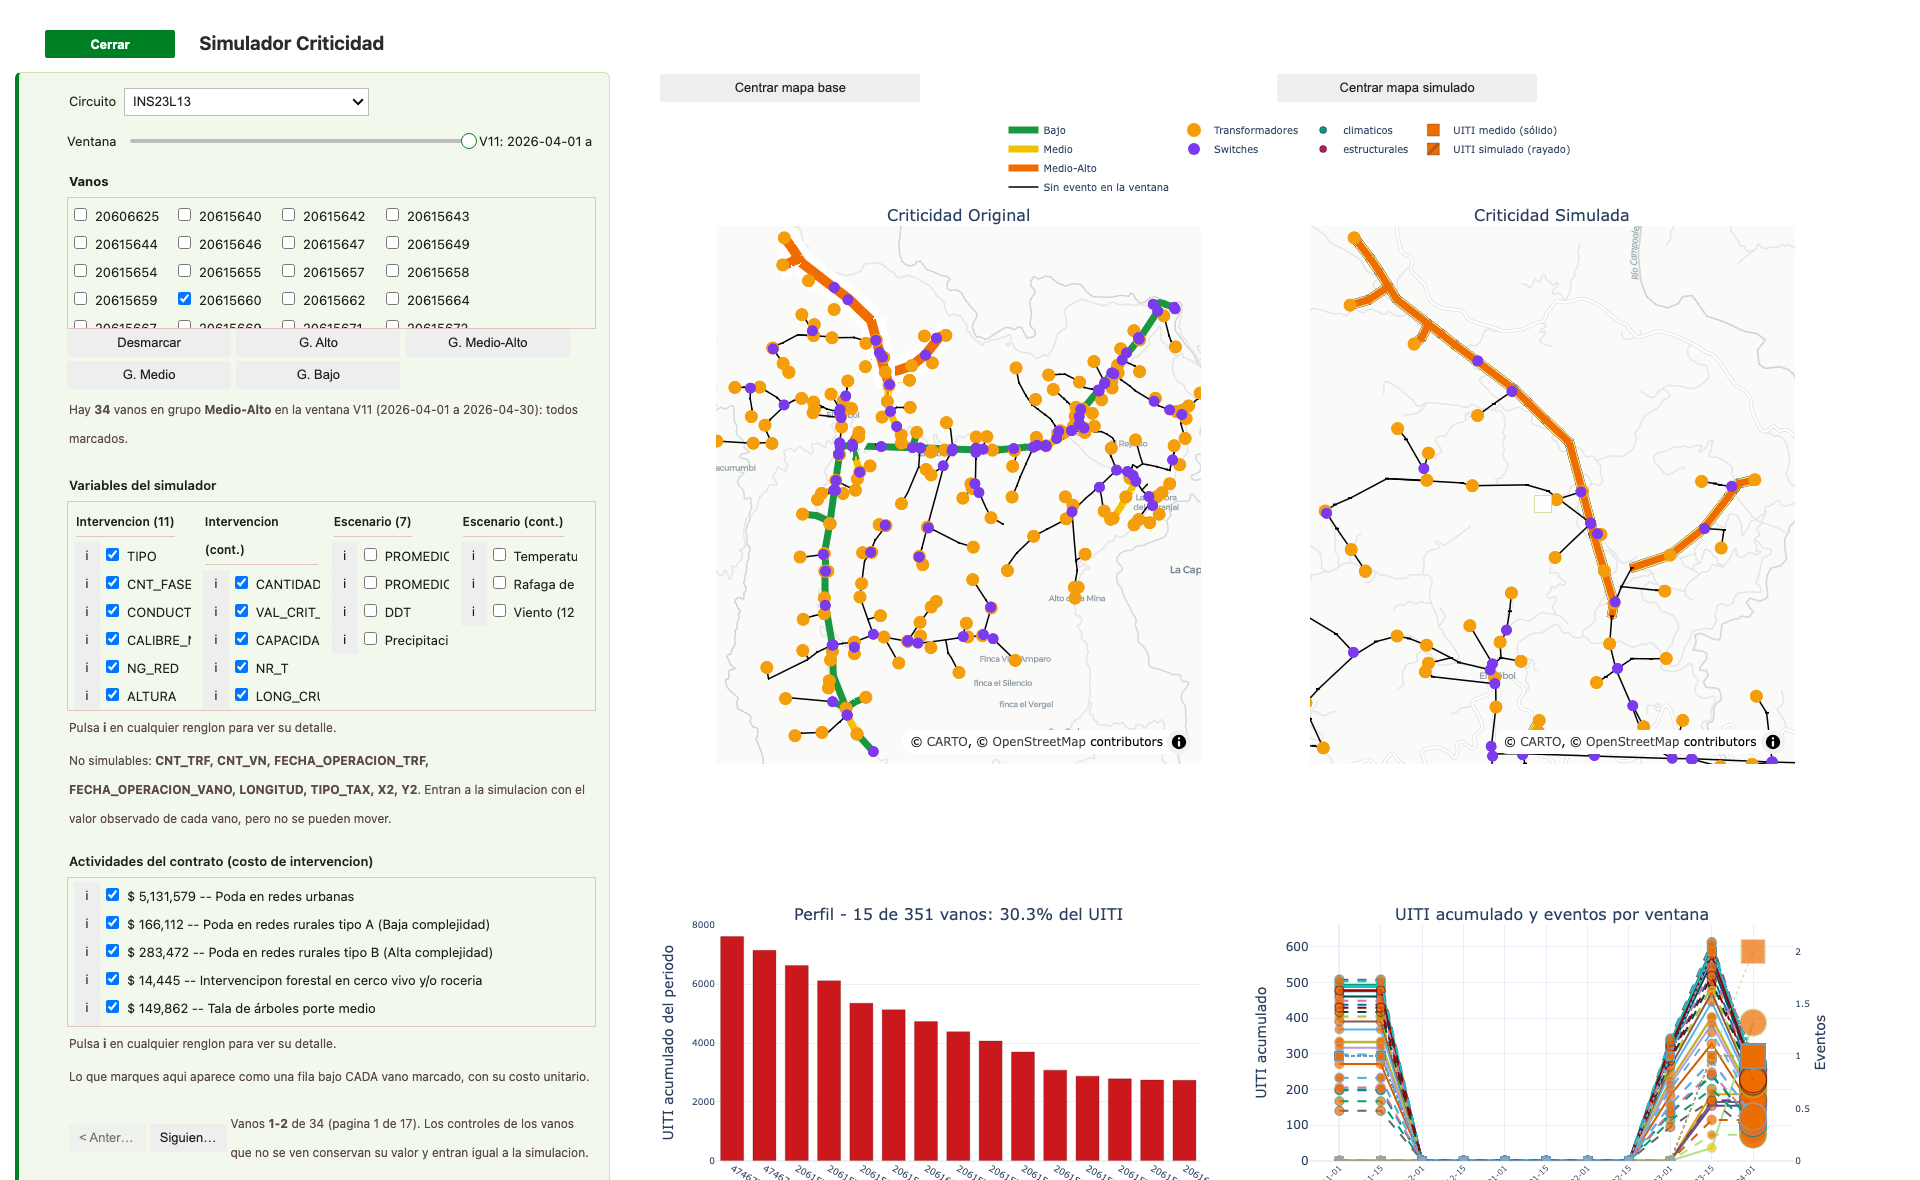
\includegraphics[width=0.96\textwidth]{figures/cuadernos/simulador_mapas.png}
\caption{Simulación contrafactual del circuito INS23L13 en la ventana V11, del 1 al 30 de abril
de 2026. Se presentan el panel de control, los mapas de criticidad original y simulada, el
perfil del circuito y la serie de UITI acumulado y eventos por ventana.}
\label{fig:simmapas}
\end{figure}

\begin{figure}[H]
\centering
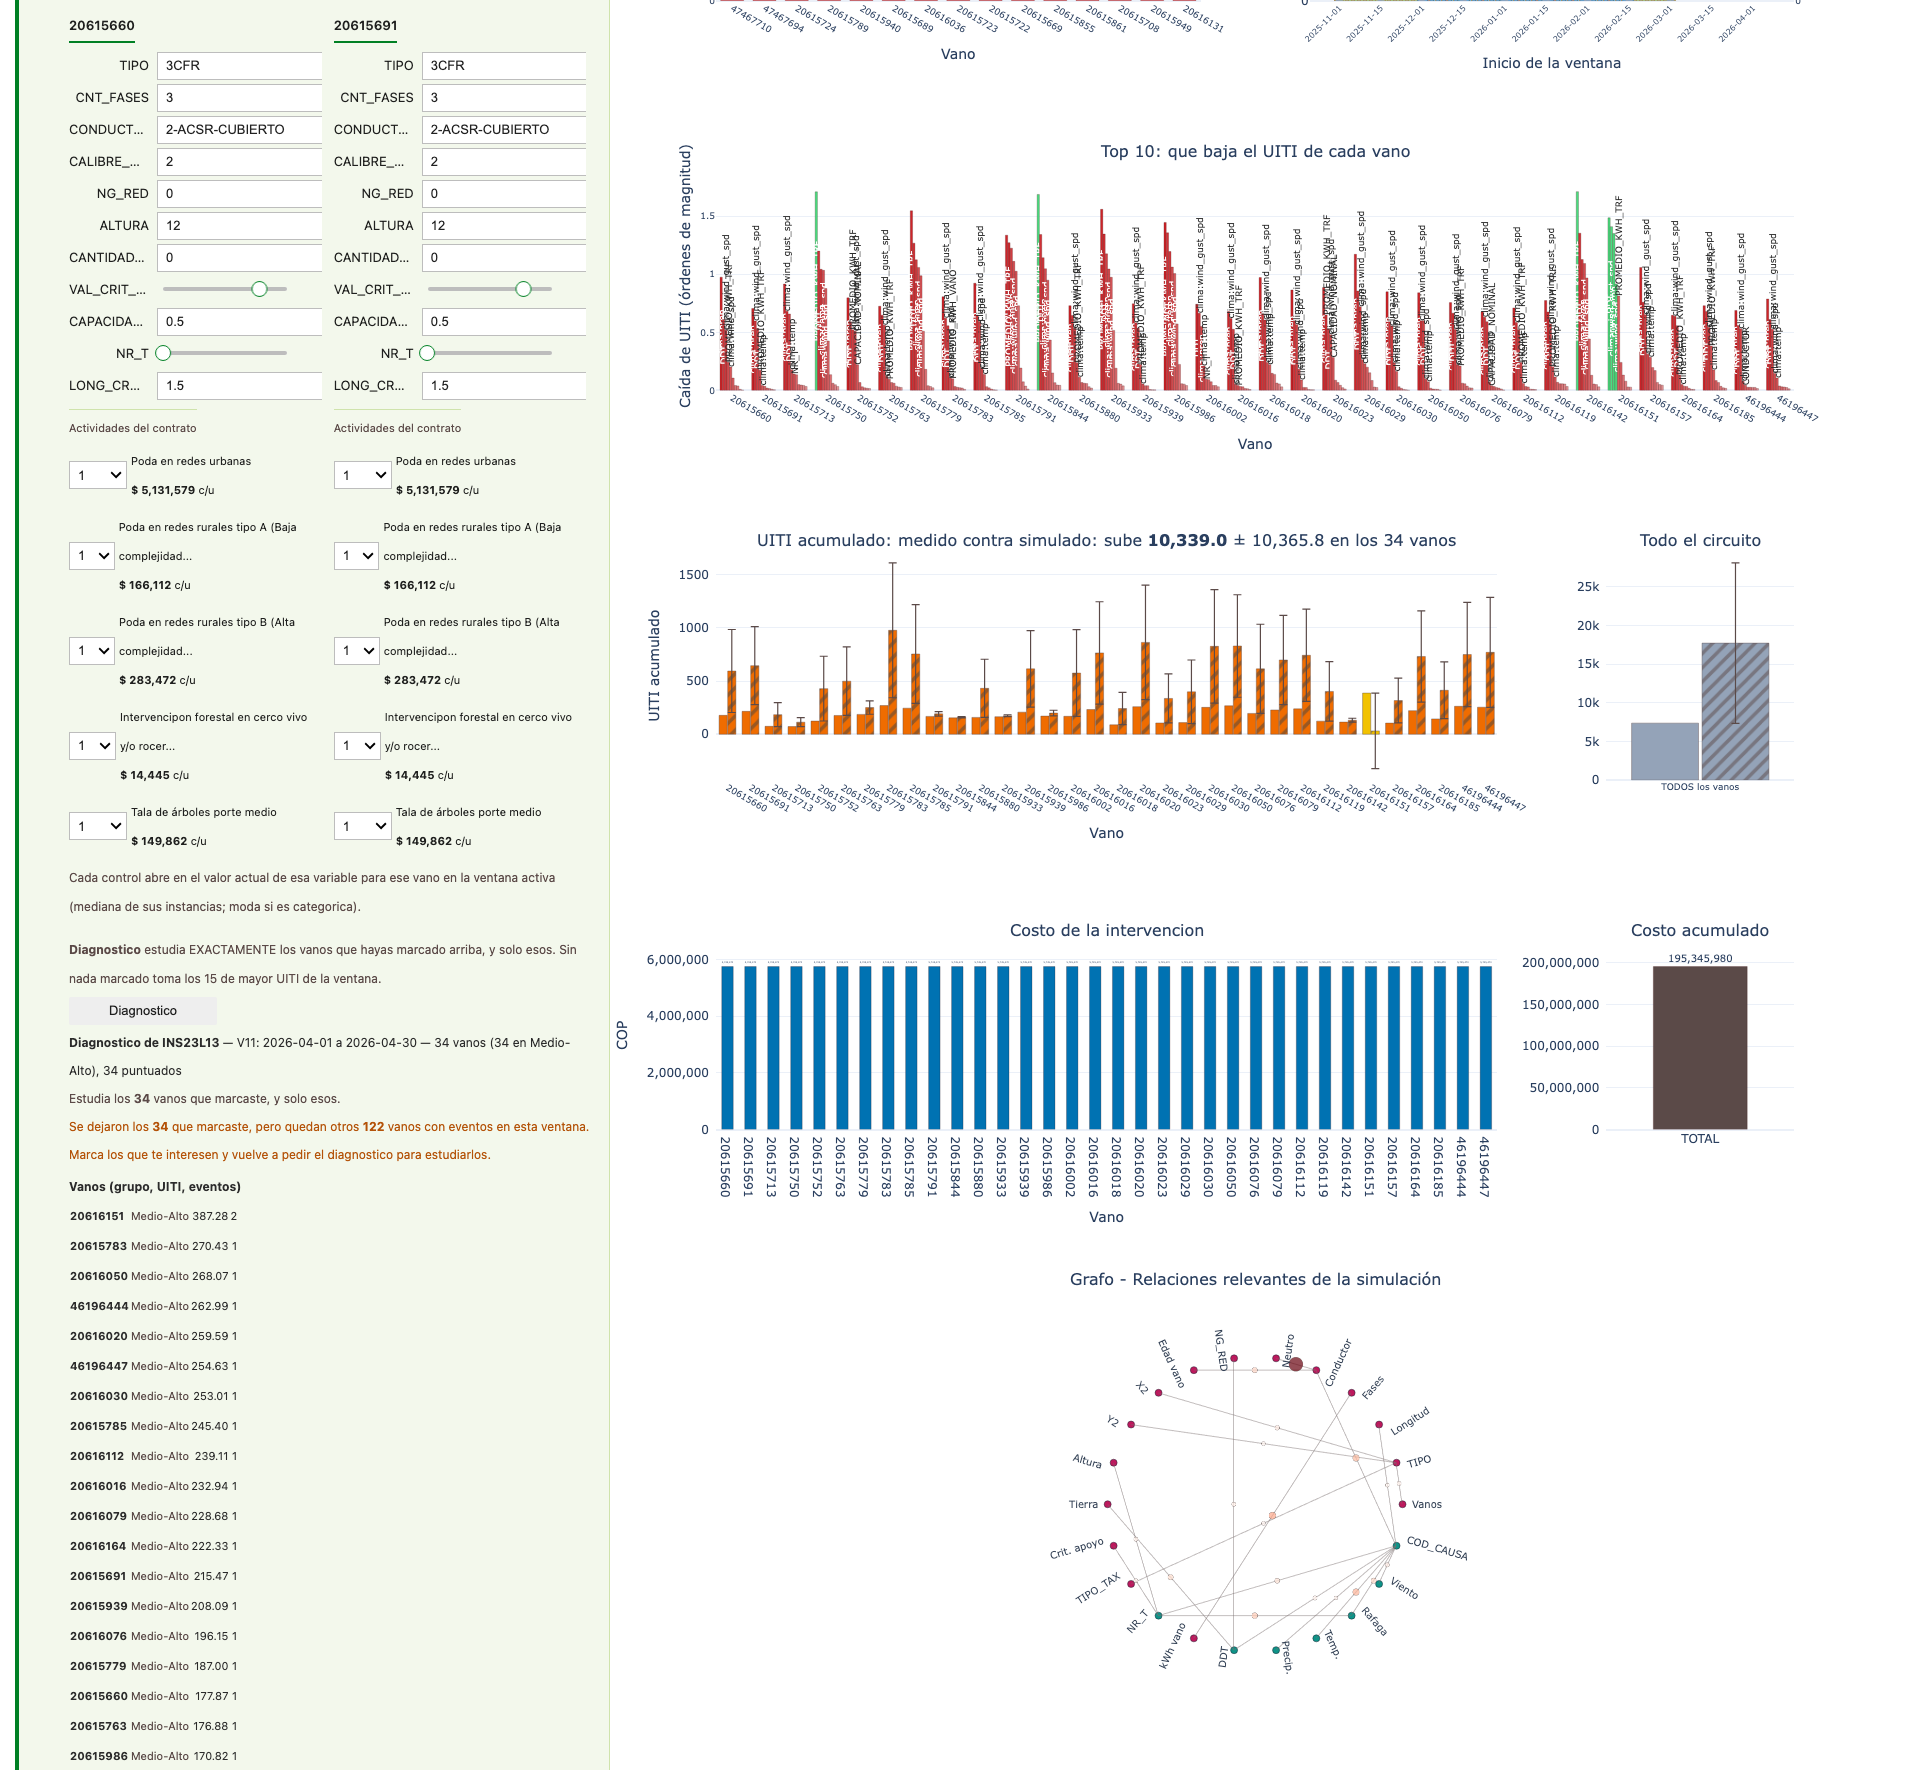
\includegraphics[width=0.96\textwidth]{figures/cuadernos/simulador_resultados.png}
\caption{Resultados de la misma ejecución: la caída de UITI que aporta cada variable en cada
vano, el UITI observado frente al simulado, el costo por vano y el costo acumulado ---
195.345.980 COP sobre cinco actividades del contrato --- y el grafo de relaciones relevantes.
El escenario simulado no produce mejora: el UITI acumulado sube $10.339{,}0$ con un desfase del
modelo de $\pm 10.365{,}8$, y el propio título del panel lo declara. Se trata de un resultado
legítimo y no de un error de ejecución: el margen es del orden del cambio, de modo que esta
corrida no sostiene una diferencia en un sentido ni en el otro. Publicar la cifra sin ese margen
convertiría el sesgo del modelo en un ahorro.}
\label{fig:simresultados}
\end{figure}

\subsection{Clases de variable y criterios de separación}

No todas las variables del modelo son modificables, y las que sí lo son no tienen el mismo
significado. El simulador las separa en tres clases, y la separación no es cosmética: determina
qué pregunta se está respondiendo. Esta capa evita que el panel presente como equivalentes
intervenciones de naturaleza distinta, por ejemplo el desplazamiento de las coordenadas
geográficas de un vano y la reducción de su riesgo por vegetación.

\begin{table}[H]
\centering
\caption{Clases de variable del simulador y criterio que las separa}
\label{tab:clasesvariable}
\footnotesize
\begin{tabularx}{\textwidth}{L{2.6cm} L{5.2cm} X}
\toprule
\textbf{Clase} & \textbf{Variables} & \textbf{Criterio} \\
\midrule
\textbf{Intervención}\newline 11 variables &
\texttt{TIPO}, \texttt{CNT\_FASES}, \texttt{CONDUCTOR}, \texttt{CALIBRE\_NEUTRO},
\texttt{NG\_RED}, \texttt{ALTURA}, \texttt{CANTIDAD\_TIERRA}, \texttt{VAL\_CRIT\_APOYO},
\texttt{CAPACIDAD\_NOMINAL}, \texttt{NR\_T}, \texttt{LONG\_CRUCETA} &
Atributos del activo que CHEC puede modificar mediante una obra. Cada una corresponde a una
actividad ejecutable del contrato --- cambio de conductor, elevación del apoyo, mejora de la
puesta a tierra o poda ---. Una variable sin obra asociada que la modifique no se considera de
intervención. \\
\addlinespace
\textbf{Escenario}\newline 7 variables &
\texttt{DDT}, precipitación, temperatura, viento y ráfaga (con 12 rezagos cada una),
\texttt{PROMEDIO\_KWH\_TRF}, \texttt{PROMEDIO\_KWH\_VANO} &
Condiciones del entorno y de la demanda que no son controlables mediante una intervención
operativa, pero que sí pueden suponerse. Combinarlas con las de intervención podría atribuir a
una obra un efecto derivado en realidad de condiciones ambientales favorables, de modo que se
simulan por separado y el tablero indica cuál de los dos componentes se aplicó. \\
\addlinespace
\textbf{No modificables}\newline 8 variables &
\texttt{CNT\_TRF}, \texttt{CNT\_VN}, \texttt{FECHA\_OPERACION\_TRF},
\texttt{FECHA\_OPERACION\_VANO}, \texttt{LONGITUD}, \texttt{TIPO\_TAX}, \texttt{X2},
\texttt{Y2} &
Ingresan a la simulación con el valor observado de cada vano, porque el modelo las requiere,
pero no admiten modificación: son atributos de identidad, contexto o topología. Modificarlas no
simula una intervención sino una entidad distinta, y reduciría la validez interpretativa del
resultado. \\
\bottomrule
\end{tabularx}
\end{table}

\subsection{Incorporación de los costos por actividad de contrato}
\label{sec:costos}

La valoración económica se apoya en un único insumo, el libro de precios del contrato de CHEC
--- \texttt{Actividades\_mantenimiento\_costos\_2026.xlsx} ---, que aporta 142 actividades con su
costo unitario en pesos colombianos. Ese archivo se lee mediante un módulo específico y no con
una lectura directa de hoja de cálculo, porque es la exportación de una tabla dinámica y
requiere tres correcciones deterministas: descartar la fila de total general, que ofrecida como
actividad introduciría el promedio de todo el catálogo; apartar y enumerar de forma explícita
las doce actividades que llegan sin costo unitario, en lugar de omitirlas en silencio; y reparar
la codificación de los nombres, dado que el catálogo carece de código de ítem y el nombre opera
como clave.

\begin{figure}[H]
\centering
\begin{tikzpicture}[node distance=8mm and 12mm]
  \node[blkn] (cat) {\textbf{Catálogo del contrato}\\ 142 actividades con su\\ costo unitario en COP};
  \node[blkd, right=of cat] (asig) {\textbf{Asignación manual}\\ el usuario marca qué actividades\\ corresponden a la intervención};
  \node[blkg, below=of cat] (fila) {\textbf{Una fila bajo cada vano}\\ con su cantidad editable:\\ cantidad $\times$ costo unitario};
  \node[blko, below=of asig] (tot) {\textbf{Costo por vano y acumulado}\\ se lee al lado de la caída\\ de UITI que lo acompaña};
  \draw[fl] (cat) -- (asig);
  \draw[fl] (asig) -- (tot);
  \draw[fl] (tot) -- (fila);
\end{tikzpicture}
\caption{Incorporación de los costos por actividad. El modelo no deduce qué actividad
corresponde a cada modificación: la asignación es del usuario.}
\label{fig:costos}
\end{figure}

El propósito del simulador no es aproximar por cercanía textual, sino cotizar el plan que el
usuario declara. La rejilla del panel recibe las actividades marcadas por vano con sus
repeticiones y devuelve el total de cada vano junto con su desglose ordenado de mayor a menor
subtotal. Un vano sin actividades conserva su fila con valor cero, porque ese cero indica que la
simulación movió su riesgo sin obra asociada. Una actividad ausente del catálogo interrumpe el
cálculo en lugar de valorarse en cero, dado que un presupuesto incompleto no sería distinguible
en pantalla de uno correcto.

\textbf{Las dos mitades permanecen deliberadamente desacopladas}: seleccionar una actividad de
poda no modifica la variable de riesgo por vegetación, y reducir esa variable no programa una
poda. El modelo no dispone de una correspondencia entre actividades contractuales y variables, y
establecerla sin respaldo produciría una cifra con apariencia de estimación de beneficio que no
lo sería. Lo que el sistema presenta lado a lado es el efecto simulado y el costo cotizado del
plan declarado; la unión de ambos permanece como decisión del usuario hasta que CHEC provea esa
correspondencia.

Los importes que el sistema despliega proceden en su totalidad del libro de precios vigente y se
recalculan en cada ejecución. El presente informe no los reproduce, dado que la cuantificación
final depende de cantidades, alcance de obra, zona, disponibilidad operativa y validación
contractual de CHEC.

\subsection{Archivo y recuperación de una simulación}
\label{sec:guardar}

Bajo los controles de simular y limpiar, el panel dispone de las acciones de guardar y cargar.
La acción de guardar permanece deshabilitada mientras no exista una simulación en pantalla,
dado que archivar un tablero vacío no constituye un registro.

\begin{figure}[H]
\centering
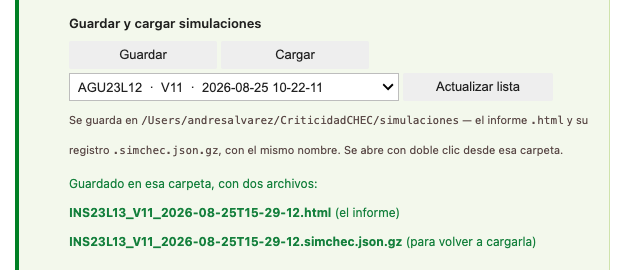
\includegraphics[width=0.86\textwidth]{figures/cuadernos/simulador_guardar.png}
\caption{Bloque de archivo del simulador. La ruta de la carpeta se publica de forma permanente
--- desde la apertura del tablero y con independencia de que se haya guardado --- en el renglón
situado bajo la lista desplegable. Tras guardar se indican los nombres de los dos archivos
escritos.}
\label{fig:simguardar}
\end{figure}

Cada ejecución archivada produce dos archivos con el mismo nombre y distinta extensión.

\begin{table}[H]
\centering
\caption{Archivos que produce la acción de guardar, con tamaños medidos sobre la ejecución de
las Figuras~\ref{fig:simmapas} y~\ref{fig:simresultados}}
\label{tab:archivos}
\footnotesize
\begin{tabularx}{\textwidth}{L{4.6cm} r X}
\toprule
\textbf{Archivo} & \textbf{Tamaño} & \textbf{Contenido} \\
\midrule
\texttt{<circuito>\_<ventana>\_}\-\texttt{<fecha>.html} & 7,1 MB &
El informe: los ocho paneles de la simulación, más tres tablas --- los vanos con las variables
simuladas y su valor fijado; las actividades de contrato por vano con número de intervenciones,
costo unitario, descripción y costo total; y el UITI medido frente al simulado por vano, con su
porcentaje de variación y los totales de ambas columnas ---. Es autocontenido: incorpora la
biblioteca de graficación, por lo que se abre sin conexión y sin requerir instalación. \\
\addlinespace
\texttt{<circuito>\_<ventana>\_}\-\texttt{<fecha>.simchec.json.gz} & 6,9 KB &
El registro con el que la acción de cargar reconstruye la simulación: circuito, ventana, los
vanos seleccionados, las variables con su valor y las actividades con sus cantidades. \\
\bottomrule
\end{tabularx}
\end{table}

\textbf{El registro no almacena las figuras}, y esa es la razón de la diferencia de tres órdenes
de magnitud entre ambos archivos. La totalidad de lo que se presenta en pantalla se deriva de
ejecutar el modelo sobre las entradas, de modo que almacenarlo equivaldría a guardar el valor de
retorno de una función junto a sus argumentos: dos representaciones de lo mismo que divergen en
el momento en que se reentrena el modelo. El registro almacena las entradas, y la acción de
cargar las repone y vuelve a ejecutar el modelo.

El costo de esa decisión --- que un modelo reentrenado devuelva valores distintos --- se asume de
forma explícita: el registro incorpora la firma criptográfica de los artefactos con los que se
ejecutó, y al cargar el panel advierte cuando no coinciden. El informe HTML, por su parte,
conserva de forma íntegra lo que se decidió ese día. El formato es gzip de JSON y no un formato
propietario, de modo que una auditoría posterior puede abrirlo sin este programa.

\begin{table}[H]
\centering
\caption{Destino de las simulaciones archivadas según el entorno de ejecución}
\label{tab:destinos}
\footnotesize
\begin{tabularx}{\textwidth}{L{2.4cm} L{5.4cm} X}
\toprule
\textbf{Entorno} & \textbf{Dónde se almacena} & \textbf{Cómo se recupera} \\
\midrule
Local, macOS y Windows &
\texttt{\textasciitilde/CriticidadCHEC/simulaciones}, o bien
\texttt{C:\textbackslash Users\textbackslash <usuario>\textbackslash}\-\texttt{CriticidadCHEC\textbackslash simulaciones} &
El informe se abre con doble clic. La carpeta depende del directorio personal del usuario y no
de la aplicación: esta se reconstruye automáticamente cuando cambian los datos y en Windows
puede trasladarse a una ruta más corta, de modo que el trabajo del usuario no debe residir en
ella. \\
\addlinespace
Databricks &
\texttt{/Volumes/<catálogo>/<esquema>/} \texttt{chec-simulador/simulaciones} &
Se descarga desde la sección de volúmenes del catálogo, en la interfaz del espacio de trabajo.
La aplicación no puede ofrecer la descarga directamente, porque el servidor que la publica no
sirve archivos individuales. \\
\bottomrule
\end{tabularx}
\end{table}

El almacenamiento en el Volume y no en el contenedor es una condición necesaria: el disco del
contenedor es efímero --- se elimina en el siguiente despliegue --- y el usuario no dispone de
acceso a él. La selección entre ambos destinos la determina una variable de entorno que el
comando de despliegue resuelve y registra en la configuración de la aplicación; no se infiere
del entorno de ejecución, dado que una inferencia de ese tipo produciría un tablero local
intentando escribir en un Volume inexistente. La carpeta se crea durante el despliegue y es
hermana de la del paquete precalculado, nunca interna a ella: el paquete se elimina y se vuelve
a crear en cada despliegue, por lo que ubicar las simulaciones en su interior eliminaría el
trabajo almacenado en cada actualización. La aplicación requiere el privilegio de escritura
sobre ese Volume; sin él, el tablero opera con normalidad y únicamente falla la acción de
guardar.

\subsection{Rendimiento medido}

La implementación no establece un límite explícito de vanos seleccionados; el rendimiento
depende de los recursos disponibles, y el diagnóstico, la aplicación de recomendaciones y los
informes cubren todos los vanos seleccionados. La prueba de mayor tamaño registrada corresponde
al circuito DON23L13 con 407 vanos: $4{,}0$~s de selección, $2{,}8$~s de diagnóstico y $5{,}8$~s
de aplicación, con 4.477 controles habilitados.

% ============================================== 9. AGENTES ================
\section{Agentes e informes automáticos}
\label{sec:agentes}

El simulador proporciona la exploración interactiva; los agentes generan la documentación
técnica de los resultados. Ambos componentes utilizan el mismo motor analítico: el diagnóstico
que el simulador muestra en pantalla --- la reducción del UITI que aporta cada variable en cada
vano --- es exactamente el que recibe y redacta el rol \texttt{inference}. Los agentes
complementan la salida del tablero con contexto histórico, análisis de informes técnicos en PDF
y comparación de evidencia.

\subsection{Qué es una habilidad y cómo se ejecuta}

Una \emph{habilidad} es un contrato declarativo en formato Markdown, versionado en el
repositorio bajo \texttt{.claude/skills/}, que especifica a un agente su tarea, sus insumos, sus
restricciones y la forma exacta del resultado esperado. No constituye código ejecutable: es la
especificación que el entorno de agente carga previamente al razonamiento.

Esa separación es la que hace verificable el sistema. El cálculo lo realiza Python de forma
determinista y la habilidad gobierna únicamente la interpretación, sujeta a tres reglas
transversales:

\begin{itemize}
  \item \textbf{Restricción al contexto entregado.} La habilidad solo puede citar fechas,
        variables, escenarios y puntos críticos contenidos en el paquete de contexto; una
        referencia ausente de ese paquete no puede figurar en su salida.
  \item \textbf{Forma de salida fijada.} Cada habilidad de razonamiento declara un contrato
        JSON con secciones obligatorias, que se valida antes de integrarse al informe. Si tras
        los reintentos de reparación no existe un objeto válido, el flujo detiene la generación
        del informe en lugar de publicar una salida que incumpla el contrato.
  \item \textbf{Invocación por referencia.} Una habilidad que requiere a otra la invoca en
        lugar de replicar su lógica, de modo que una modificación del motor de reporte se
        propaga a todos sus consumidores sin sincronización manual.
\end{itemize}

\subsection{Informe por circuito}

\begin{figure}[H]
\centering
\begin{tikzpicture}[node distance=6mm and 9mm]
  \node[blkn] (ins) {\textbf{Insumos}\\ datos estructurados $\cdot$ artefacto \texttt{.pt}\\ informes expertos en PDF $\cdot$ bóveda del circuito};
  \node[blkg, below=8mm of ins] (prep) {\texttt{prepare}\\ determinista, sin modelo de lenguaje:\\ arma el contexto};
  \node[blkd, below=9mm of prep, xshift=-52mm] (h) {1 $\cdot$ \texttt{historical}\\ diagnóstico descriptivo\\ de la serie};
  \node[blkd, below=9mm of prep] (i) {2 $\cdot$ \texttt{inference}\\ lee el modelo: relevancia\\ por vano y plan};
  \node[blkd, below=9mm of prep, xshift=52mm] (e) {3 $\cdot$ \texttt{expert-alignment}\\ coteja el modelo contra\\ la discusión experta};
  \node[blko, below=9mm of i] (ren) {\texttt{render}\\ informe HTML del circuito};
  \node[blk, below=7mm of ren] (vau) {nota de bóveda $+$ grafo\\ alimenta la próxima ejecución};
  \draw[fl] (ins) -- (prep);
  \draw[fl] (prep) -- (h);
  \draw[fl] (prep) -- (i);
  \draw[fl] (prep) -- (e);
  \draw[fl] (h.south) |- (ren.west);
  \draw[fl] (i) -- (ren);
  \draw[fl] (e.south) |- (ren.east);
  \draw[fl] (ren) -- (vau);
  \draw[fld] (vau.west) -- ++(-7.2,0) |- ([yshift=-2mm]ins.west);
\end{tikzpicture}
\caption{Flujo del informe por circuito. La preparación y el renderizado son deterministas y se
ejecutan sin modelo de lenguaje; únicamente los tres roles intermedios lo utilizan. La nota de
bóveda que produce cada corrida alimenta la siguiente.}
\label{fig:report}
\end{figure}

\begin{table}[H]
\centering
\caption{Roles de agente: insumo, función y producto}
\label{tab:agentes}
\footnotesize
\begin{tabularx}{\textwidth}{L{3.4cm} L{3.6cm} X}
\toprule
\textbf{Rol} & \textbf{Insumo} & \textbf{Producto} \\
\midrule
\texttt{historical} &
Selección de circuito y ventana, serie diaria, puntos críticos, causas observadas, variables
disponibles y faltantes, y relaciones del grafo. &
Objeto JSON con el diagnóstico descriptivo del comportamiento de \texttt{UITI\_VANO}:
secciones de análisis, referencias a fechas y puntos críticos existentes, hipótesis históricas y
limitaciones declaradas. \\
\addlinespace
\texttt{inference} &
Relevancia por vano y por variable derivada del modelo, escenarios por ventana, puntajes por
modo y metadatos del artefacto. &
Objeto JSON con la interpretación predictiva por escenario. No puede priorizar
\texttt{UITI\_VANO} como predictor ni citar escenarios que el flujo no generó, y debe declarar
que las relevancias y los grafos explican asociaciones, no causalidad. \\
\addlinespace
\texttt{expert-alignment} &
Los dos objetos JSON validados anteriores, las filas expertas ya filtradas por cercanía
temporal y la lista exacta de variables del modelo. &
Objeto JSON con coincidencias, diferencias, brechas, hasta cinco variables priorizadas para
revisión operativa y una síntesis. Solo puede citar evidencia de las filas comparadas. \\
\addlinespace
\texttt{pdf-discussion-} \texttt{extraction} &
Un fragmento de informe técnico con sus metadatos: archivo de origen, páginas, circuito
heredado del nombre del archivo, periodo y ventana solicitada. &
Decisión de incluir o descartar. Si incluye, una fila con circuito, fecha o intervalo
normalizado, análisis breve y evidencia textual del propio fragmento. \\
\bottomrule
\end{tabularx}
\end{table}

\subsection{Informe gerencial por banda de riesgo}

La síntesis transversal parte de una banda de riesgo de la clasificación descrita en la
Sección~\ref{sec:bandas}. Si la banda contiene más de doce circuitos se toman los doce más
críticos, y el informe declara de forma explícita que \textbf{describe la cola de la banda y no
su circuito típico}. El panorama que sintetiza tiene por universo el grupo completo, nunca la
muestra: las barras del conjunto abarcan los 208 circuitos con la muestra resaltada, y el grafo
radial de causas reúne los patrones que cruzan circuitos.

\begin{table}[H]
\centering
\caption{Comandos de informe y de datos, con su alcance}
\label{tab:comandosinforme}
\small
\begin{tabularx}{\textwidth}{L{3.4cm} X L{4.0cm}}
\toprule
\textbf{Comando} & \textbf{Salida generada} & \textbf{Alcance} \\
\midrule
\texttt{/report} & Informe HTML de un circuito, con figuras y trazabilidad por afirmación. & Un circuito, una ventana. \\
\texttt{/reporte-lote} & Encadena \texttt{/report} sobre una lista de circuitos. & Varios circuitos. \\
\texttt{/informe-gerencial} & Síntesis por banda de riesgo, con barras del conjunto completo de circuitos y grafo radial de causas. & Hasta 12 circuitos de una banda. \\
\texttt{/clima} & Enriquece los datos con Open-Meteo, bajo tres validaciones de cuota. & Toda la tabla elegida. \\
\texttt{/vault-circuito} & Proyecta el circuito a una nota Markdown e indexa el grafo de conocimiento. & Acumulativo entre ejecuciones. \\
\bottomrule
\end{tabularx}
\end{table}

\paragraph{Costo por informe.} Un informe por circuito consume del orden de 318.760 unidades de
texto del modelo de lenguaje. El requisito determinante no es la capacidad de cómputo local sino
\textbf{la cuota del modelo}: mientras los tres roles razonan, el equipo permanece ocioso.

% ============================================== 10. DATABRICKS ============
\section{Migración a Azure Databricks}
\label{sec:databricks}

El despliegue en Databricks es independiente y no mantiene sincronización en tiempo real con el
entorno local: allí se ejecuta la misma cadena, con sus propios datos cargados y sus propias
aplicaciones desplegadas. La migración se ejecuta mediante un único comando,
\texttt{/subir-a-databricks}, que transfiere tres grupos de artefactos.

\subsection{La interfaz de línea de comandos como estrategia central}

El uso de la interfaz de línea de comandos de Databricks no constituye un detalle de
implementación: es el mecanismo que permite a un agente de código conducir el despliegue
completo desde la terminal, sin recurrir a la interfaz web del espacio de trabajo. El comando se
comunica con Databricks exclusivamente por esa vía --- 51 invocaciones ---: la apertura de sesión
por OAuth, el descubrimiento del catálogo y del Volume, la copia de archivos, la importación del
cuaderno y la creación y despliegue de las aplicaciones. De ahí que el usuario solo aporte la
URL del espacio de trabajo: el perfil se deriva de esa URL y todo lo demás se resuelve en tiempo
de ejecución.

\begin{table}[H]
\centering
\caption{Artefactos que transfiere el despliegue}
\label{tab:artefactos}
\small
\begin{tabularx}{\textwidth}{c L{4.4cm} L{3.4cm} X}
\toprule
\textbf{\#} & \textbf{Artefacto} & \textbf{Destino} & \textbf{Contenido} \\
\midrule
1 & \texttt{data/} & Volume de Unity Catalog &
Aproximadamente 945 MB: el archivo de eventos (566), la caché de bolsas (199), los tres
archivos geográficos con sus complementos (180), el modelo entrenado, el grafo y los catálogos
en hoja de cálculo. \\
\addlinespace
2 & Dos aplicaciones & Databricks Apps, cada una en su recurso de cómputo &
La aplicación de criticidad sirve los cuatro tableros en cuatro rutas; el simulador requiere un
intérprete de Python en ejecución. \\
\addlinespace
3 & \texttt{notebooks/05\_mil\_vano\_} \texttt{ventana.ipynb} & Cuaderno del espacio de trabajo &
El registro legible del modelo, importado sin salidas por el tope de 10 MB del importador. \\
\bottomrule
\end{tabularx}
\end{table}

\subsection{Secuencia de ejecución}

El comando solicita un solo dato al usuario --- la URL del espacio de trabajo de destino --- y
todo lo demás se resuelve o se descubre en tiempo de ejecución.

\begin{table}[H]
\centering
\caption{Las ocho etapas de \texttt{/subir-a-databricks}}
\label{tab:etapas}
\footnotesize
\begin{tabularx}{\textwidth}{c L{5.0cm} X}
\toprule
\textbf{\#} & \textbf{Etapa} & \textbf{Comportamiento} \\
\midrule
1 & Solicitud de la URL del espacio de trabajo &
Es el único dato que se solicita, y se solicita en cada ejecución: nunca se deduce de un perfil
con sesión abierta, dado que un destino incorrecto no produce ningún error observable. \\
2 & Resolución del perfil y de la identidad & Se derivan de esa URL, una sola vez, y la identidad se confirma con una llamada real antes de transferir datos. \\
3 & Resolución del destino en Unity Catalog & El catálogo se descubre en tiempo de ejecución; nunca se asume. \\
4 & Validación de los datos en el Volume &
Se verifican primero los archivos existentes y sus tamaños. Solo se transfieren los faltantes:
retransmitir los 566 MB ya presentes es la operación más costosa del proceso. \\
5 & Validación de las aplicaciones &
Una aplicación se considera operativa cuando su estado es activo, su proceso está en ejecución
y su último despliegue fue satisfactorio, de forma simultánea. Una aplicación operativa y
actualizada no requiere un nuevo despliegue. \\
6 & Validación del cuaderno &
Se importa sin salidas ni contadores de ejecución. Si la etapa de datos quedó bloqueada, el
cuaderno queda disponible pero no podrá ejecutarse: esa condición se registra como
\emph{degradado}, no como satisfactoria. \\
7 & Registro y publicación de la bitácora & En una rama, nunca sobre la rama principal. \\
8 & Generación del reporte de ejecución & Una fila por etapa, la ruta de la bitácora y cada restricción junto con el responsable de su resolución. \\
\bottomrule
\end{tabularx}
\end{table}

\subsection{Trazabilidad del despliegue}

La etapa final produce dos tablas cuyo propósito es que una corrida quede auditable sin releer
la salida de la terminal.

La primera resume el proceso con una fila por etapa --- siempre las tres etapas de transferencia,
incluso las que no hicieron falta o quedaron bloqueadas ---, con columnas de lo que ya estaba, lo
que se subió, el estado y \textbf{la causa}. La columna de causa la llenan únicamente las etapas
que no terminaron de forma satisfactoria, e indica \emph{por qué}, no \emph{qué}. Una etapa que
no salió bien y no declara causa se reporta de forma explícita como carente de causa registrada:
una celda vacía junto a un fallo se leería como un fallo sin motivo, y eso constituiría otra
afirmación.

La segunda es la tabla de ubicaciones, que responde la pregunta que se formula cuando el
despliegue salió bien: dónde quedó cada cosa. Reúne el Volume de datos, el paquete precalculado
del simulador, la carpeta de simulaciones guardadas, las dos aplicaciones con su URL literal y
el cuaderno del espacio de trabajo, cada uno con su ruta y su camino de acceso en la interfaz.
Esas rutas no son deducibles, porque el catálogo y el esquema se resuelven en cada corrida.

La bitácora se escribe en formato Markdown bajo \texttt{reports/despliegues/} y sanea de su
contenido cualquier credencial --- tokens de acceso, secretos de cliente y contraseñas --- antes
de registrarla. El despliegue no modifica ningún cuaderno del repositorio y no integra nada en
la rama principal.

% ============================================== 11. INSTALACION ===========
\section{Instalación y puesta en marcha}
\label{sec:instalacion}

La puesta en marcha se compone de seis pasos, de los cuales los dos últimos aplican únicamente
si el proyecto se despliega en Databricks. Los pasos 3, 4 y 6 se ejecutan desde un agente de
código y no requieren instalar dependencias a mano.

\subsection{Los seis pasos}

\begin{enumerate}
  \item \textbf{Clonar el repositorio}, con \texttt{git lfs} instalado \emph{antes} de clonar:
        \texttt{git lfs install}, luego \texttt{git clone} y, dentro de la carpeta,
        \texttt{git lfs pull}. Este último paso no es opcional: sin él, la base de eventos de
        566 MB y la caché de bolsas de 199 MB se descargan como punteros de 134 bytes, que
        existen en el sistema de archivos y no contienen datos, de modo que el fallo se
        manifiesta mucho después y sin referencia a esta causa. En Windows, la ruta del clon
        debe caber en 61 caracteres; el repositorio incluye un guion que lo resuelve sin
        requerir permisos administrativos.

  \item \textbf{Abrir el agente de código.} Todo lo que sigue se ejecuta desde un agente. El
        repositorio publica sus quince comandos para tres entornos --- Claude Code, que es la
        fuente del contrato, OpenCode y VS Code Copilot --- y la invocación es idéntica en los
        tres. Se abre el agente de preferencia en la carpeta del clon.

  \item \textbf{Instalar dependencias con \texttt{/instalar-local}.} El comando ejecuta primero
        un diagnóstico con el intérprete de Python del sistema y solo la biblioteca estándar,
        dado que debe funcionar en un clon donde aún no existe ningún entorno: devuelve
        dieciséis comprobaciones con el comando de corrección correspondiente al sistema
        operativo detectado. A continuación solicita \textbf{un único dato} --- cuál de los tres
        destinos debe quedar operativo: el cuaderno de entrenamiento, las aplicaciones locales o
        el despliegue en Databricks --- y solo entonces instala, en el orden de dependencia: los
        datos de LFS, el entorno raíz, los seis entornos de las aplicaciones y la interfaz de
        línea de comandos de Databricks. \textbf{Los componentes ya presentes no se modifican.}

  \item \textbf{Verificar que los tableros y el simulador operan.} Un diagnóstico satisfactorio
        no equivale a haber iniciado un tablero. La comprobación se realiza con
        \texttt{/app-local-criticidadCHEC}, o mediante doble clic sobre la aplicación del menú:
        este abre en el puerto 8800 y desde él se inician los cuatro tableros estáticos (8801 a
        8804) y el simulador (8866). \textbf{El simulador constituye la verificación
        determinante}, por ser el único componente que requiere un intérprete de Python en
        ejecución: marcar un vano y ejecutar una simulación confirma simultáneamente que el
        entorno está completo, que el modelo carga y que el navegador mantiene la comunicación
        con el núcleo de cómputo.

  \item \textbf{Instalar la interfaz de línea de comandos de Databricks}, únicamente para el
        despliegue. Al seleccionar ese destino, \texttt{/instalar-local} la instala y verifica
        su compatibilidad: no se limita a comprobar su presencia, sino que valida que la
        creación de aplicaciones acepte el parámetro de tamaño de cómputo, dado que una versión
        antigua completa las etapas iniciales y falla durante el despliegue. La sesión la abre
        el usuario con \texttt{databricks auth login -{}-host <URL>}, por requerir el navegador.
        El comando de instalación \textbf{no establece comunicación con Databricks}: deja la
        interfaz instalada y la sesión activa.

  \item \textbf{Desplegar con \texttt{/subir-a-databricks}.} Es el único comando que se comunica
        con el espacio de trabajo. Solicita un solo dato --- su URL, del tipo
        \texttt{https://adb-\allowbreak xxxxxxxxxxxx.\allowbreak 0.azuredatabricks.net} --- y la solicita en cada
        ejecución. De esa URL deriva el perfil y confirma la identidad con una llamada real
        antes de transferir datos. Si el token está vencido, la ejecución se detiene y solicita
        una nueva apertura de sesión. Las ocho etapas que recorre después se detallan en la
        Sección~\ref{sec:databricks}.
\end{enumerate}

\subsection{Requisitos de máquina, medidos}

Las cifras siguientes están medidas sobre el repositorio y no estimadas. El equipo de
referencia es un Apple M4 Max de 14 núcleos con 36 GB de memoria y disco de estado sólido. Lo
que no cambia entre máquinas es el orden de magnitud y qué parte resulta costosa.

\begin{table}[H]
\centering
\caption{Requisitos mínimos por componente}
\label{tab:requisitos}
\small
\begin{tabularx}{\textwidth}{X c c c L{2.6cm}}
\toprule
\textbf{Uso previsto} & \textbf{Memoria} & \textbf{Núcleos} & \textbf{Disco libre} & \textbf{Red} \\
\midrule
Solo los cuatro tableros estáticos & 4 GB & 2 & 3,5 GB & Instalación y LFS \\
Además el simulador & 8 GB & 4 & 6 GB & Instalación y LFS \\
Además reentrenar el modelo & 8 GB & 2 & $+$3 GB & LFS, una vez \\
Además generar informes con agentes & 8 GB & 4 & $+$1 GB & Permanente \\
\midrule
\textbf{Todo, con holgura} & \textbf{16 GB} & \textbf{4--8} & \textbf{20 GB} & Permanente \\
\bottomrule
\end{tabularx}
\end{table}

\textbf{Ninguna parte del proyecto requiere GPU}, según la medición reportada en la
Tabla~\ref{tab:dispositivo}. La resolución mínima de pantalla para los tableros es de
$1.280 \times 800$; por debajo siguen siendo utilizables y no desbordan, pero las figuras se
dibujan por debajo de su tamaño de diseño.

Python 3.11 constituye un piso real y no una preferencia: las versiones requeridas de las
bibliotecas numéricas no publican paquetes binarios por debajo de esa versión. El rango se ha
ejercitado en ambos extremos --- el entorno raíz en 3.11.15 y los seis de las aplicaciones en
3.14.6 ---. Ninguna dependencia exige compilador local, dado que existen paquetes binarios
precompilados para macOS y Windows de las bibliotecas de mayor tamaño.

\subsection{Las cuatro listas de dependencias}

Las dependencias se distribuyen en cuatro listas separadas. La separación es deliberada: el menú
mantiene un entorno mínimo de aproximadamente 15 MB y no carga las dependencias de los cinco
tableros, lo que evita, por ejemplo, requerir la biblioteca de aprendizaje profundo únicamente
para iniciar el menú principal.

\begin{table}[H]
\centering
\caption{Listas de dependencias por componente}
\label{tab:dependencias}
\footnotesize
\begin{tabularx}{\textwidth}{L{3.6cm} L{4.0cm} X}
\toprule
\textbf{Componente} & \textbf{Lista} & \textbf{Dependencias principales} \\
\midrule
Los cuatro tableros estáticos (8801 a 8804) &
\texttt{aplicaciones/<app>/} \texttt{requirements.txt}, una por tablero &
\texttt{pandas}, \texttt{numpy}, \texttt{scipy}, \texttt{scikit-learn}, \texttt{plotly},
\texttt{pyarrow}, \texttt{geopandas}, \texttt{shapely}, \texttt{ipython} \\
\addlinespace
El simulador (8866) &
\texttt{aplicaciones/06\_simulador/} \texttt{requirements.txt} &
Las anteriores y, adicionalmente, \texttt{torch}, \texttt{voila},
\texttt{jupyter-server}, \texttt{ipykernel}, \texttt{ipywidgets}, \texttt{anywidget},
\texttt{joblib}, \texttt{cloudpickle}, \texttt{openpyxl}, \texttt{pyogrio},
\texttt{matplotlib} \\
\addlinespace
El cuaderno de entrenamiento &
\texttt{requirements.txt} de la raíz &
\texttt{torch}, \texttt{networkx}, \texttt{jupyter}, \texttt{ipykernel},
\texttt{papermill}, \texttt{nbformat}, \texttt{pyproj}, \texttt{folium}, además de las
dependencias numéricas y geoespaciales \\
\addlinespace
Los informes con agentes &
\texttt{requirements.txt} de la raíz &
Las del cuaderno y, adicionalmente, \texttt{pdfplumber}, \texttt{jsonschema},
\texttt{xlsxwriter}, \texttt{graphifyy}, \texttt{openmeteo-requests},
\texttt{requests-cache}, \texttt{retry-requests} \\
\bottomrule
\end{tabularx}
\end{table}

La generación de informes depende principalmente de la disponibilidad del servicio de modelo de
lenguaje y de la conectividad de red, más que de recursos locales de cómputo. Es el único
componente que requiere un servicio externo no incluido en la instalación local. El resto puede
ejecutarse sin conexión una vez completada la instalación y disponibles los insumos.

\subsection{Comandos de instalación y mantenimiento}

\begin{table}[H]
\centering
\caption{Comandos que cubren el ciclo del entorno}
\label{tab:comandosentorno}
\small
\begin{tabularx}{\textwidth}{L{4.4cm} X}
\toprule
\textbf{Comando} & \textbf{Función} \\
\midrule
\texttt{/instalar-local} &
Verifica el entorno y prepara los componentes requeridos para las tres operaciones principales:
ejecutar el cuaderno de entrenamiento, iniciar el menú con sus cinco tableros y desplegar en
Databricks. Diagnostica primero --- Python, \texttt{git-lfs}, insumos, entornos, puertos, salida
al repositorio de paquetes y la interfaz de Databricks --- e instala únicamente los componentes
faltantes. Distingue macOS de Windows en cada paso. \\
\addlinespace
\texttt{/app-local-criticidadCHEC} &
Inicia el menú desde el cual se lanzan, supervisan y detienen los cinco tableros. Crea el
entorno de cada aplicación la primera vez que se requiere. \\
\addlinespace
\texttt{/actualizar} &
Detecta cambios en los insumos que afectan al modelo --- la base de eventos, el diccionario de
variables o el grafo declarado --- y reconstruye, en el orden correspondiente, los artefactos
afectados: el reentrenamiento, la geometría y los paquetes de las aplicaciones. Si no se
detectan cambios, no se ejecuta ninguna acción. \\
\bottomrule
\end{tabularx}
\end{table}

\subsection{Portabilidad entre entornos de agente}

La instalación no está atada a un proveedor de modelo ni a un editor. Los comandos son contratos
en texto --- persona, invariantes, secuencia de ejecución y forma de la salida ---, de modo que
pueden ejecutarse con distintos modelos de lenguaje según la cuota y la política de datos de la
organización.

\begin{table}[H]
\centering
\caption{Ubicación de los comandos y roles en los tres entornos de agente}
\label{tab:portabilidad}
\small
\begin{tabularx}{\textwidth}{L{3.4cm} X X}
\toprule
\textbf{Entorno} & \textbf{Comandos} & \textbf{Roles y reglas} \\
\midrule
Claude Code \newline \emph{fuente del contrato} & \texttt{.claude/skills/*/SKILL.md} y \texttt{.claude/commands/*.md} & \texttt{.claude/agents/*.md} \\
OpenCode \newline \emph{espejo generado} & \texttt{.opencode/command/*.md} & \texttt{.opencode/agent/*.md}, \texttt{AGENTS.md} \\
VS Code Copilot \newline \emph{espejo generado} & \texttt{.github/prompts/*.prompt.md} & \texttt{.github/agents/*.agent.md}, \texttt{AGENTS.md} \\
\bottomrule
\end{tabularx}
\end{table}

La fuente única es el directorio de Claude Code; los espejos se generan mediante un guion del
repositorio, de forma que un comando renombrado o retirado se propaga en una sola ejecución. La
invocación es idéntica en los tres entornos.

\begin{table}[H]
\centering
\caption{Los quince comandos publicados}
\label{tab:comandos}
\footnotesize
\begin{tabularx}{\textwidth}{L{4.6cm} X}
\toprule
\textbf{Comando} & \textbf{Función} \\
\midrule
\texttt{/actualizar} & Reconstruye lo afectado cuando cambian los insumos. \\
\texttt{/app-local-criticidadCHEC} & Abre el menú y sus cinco tableros. \\
\texttt{/clima} & Enriquece los datos con Open-Meteo. \\
\texttt{/expert-alignment} & Rol de agente: cotejo contra la discusión experta. \\
\texttt{/historical} & Rol de agente: diagnóstico descriptivo de la serie. \\
\texttt{/inference} & Rol de agente: lectura del modelo predictivo. \\
\texttt{/informe-gerencial} & Síntesis por banda, con barras y grafo radial. \\
\texttt{/instalar-local} & Diagnostica la máquina e instala lo que falta. \\
\texttt{/limpiar-corridas} & Mantenimiento de artefactos de corrida, con confirmación explícita. \\
\texttt{/pdf-discussion-extraction} & Rol de agente: tabla de discusiones desde informes en PDF. \\
\texttt{/redaccion-es} & Revisión ortográfica y de redacción de la prosa generada. \\
\texttt{/report} & Informe HTML de un circuito. \\
\texttt{/reporte-lote} & Encadena \texttt{/report} sobre una banda de riesgo. \\
\texttt{/subir-a-databricks} & Despliegue a Databricks, en ocho etapas. \\
\texttt{/vault-circuito} & Proyecta el circuito a la bóveda y encadena la construcción del grafo. \\
\bottomrule
\end{tabularx}
\end{table}

\subsection{Primer recorrido de uso}

Completada la instalación, la secuencia siguiente recorre el sistema de principio a fin y
remite a la sección que describe cada pieza.

\begin{enumerate}
  \item \textbf{Abrir el menú} con \texttt{/app-local-criticidadCHEC}. Desde él se inician y
        se detienen las cinco aplicaciones (Tabla~\ref{tab:tableros}).
  \item \textbf{Situar el problema.} El tablero de agrupamiento indica en qué vanos se
        concentra la criticidad, y el ranking de circuitos, en qué circuitos
        (Sección~\ref{sec:bandas}). De ahí sale la banda de riesgo sobre la que conviene
        trabajar.
  \item \textbf{Situarlo en el tiempo.} Los tableros de trayectorias muestran si el circuito
        elegido mejora o se deteriora y en qué ventana, primero a nivel de circuito y después
        a nivel de vano.
  \item \textbf{Revisar la condición ambiental.} El tablero climático enfrenta el UITI diario
        contra la variable meteorológica de interés y sus doce horas previas. Si se requieren
        datos nuevos, el comando \texttt{/clima} los incorpora (Tabla~\ref{tab:clima}).
  \item \textbf{Simular la intervención.} En el simulador se elige el circuito y la ventana,
        se marcan los vanos, se ejecuta el diagnóstico, se aplican o se ajustan los valores
        propuestos, se asignan las actividades de contrato y se ejecuta la simulación
        (Sección~\ref{sec:simulador}).
  \item \textbf{Archivar el resultado.} La acción de guardar deja el informe HTML y su
        registro en la carpeta de simulaciones; la de cargar repone una ejecución anterior y
        vuelve a evaluar el modelo (Sección~\ref{sec:guardar}).
  \item \textbf{Documentar.} \texttt{/report} produce el informe técnico del circuito;
        \texttt{/informe-gerencial}, la síntesis de la banda (Sección~\ref{sec:agentes}).
  \item \textbf{Publicar en la nube}, si corresponde, con \texttt{/subir-a-databricks}
        (Sección~\ref{sec:databricks}).
\end{enumerate}

Cuando cambien los insumos --- la base de eventos, el diccionario de variables o el grafo
declarado ---, \texttt{/actualizar} reconstruye en orden los artefactos afectados; las
aplicaciones, por su parte, detectan el cambio por sí solas y se reconstruyen al abrirse.

% ============================================== 12. GRAFO =================
\section{Grafo de conocimiento del proyecto}

El grafo de conocimiento del repositorio se construye sobre el código y la documentación
mediante una herramienta de indexación versionada junto al proyecto. El grafo completo comprende
9.976 nodos y 17.025 aristas, cantidad que dificulta su inspección simultánea, por lo que se
publica su vista agregada: 754 comunidades y las 877 relaciones entre ellas. Cada punto
corresponde a un grupo de símbolos que el algoritmo identificó como unidos, y el número asociado
indica cuántos símbolos contiene.

\begin{figure}[H]
\centering
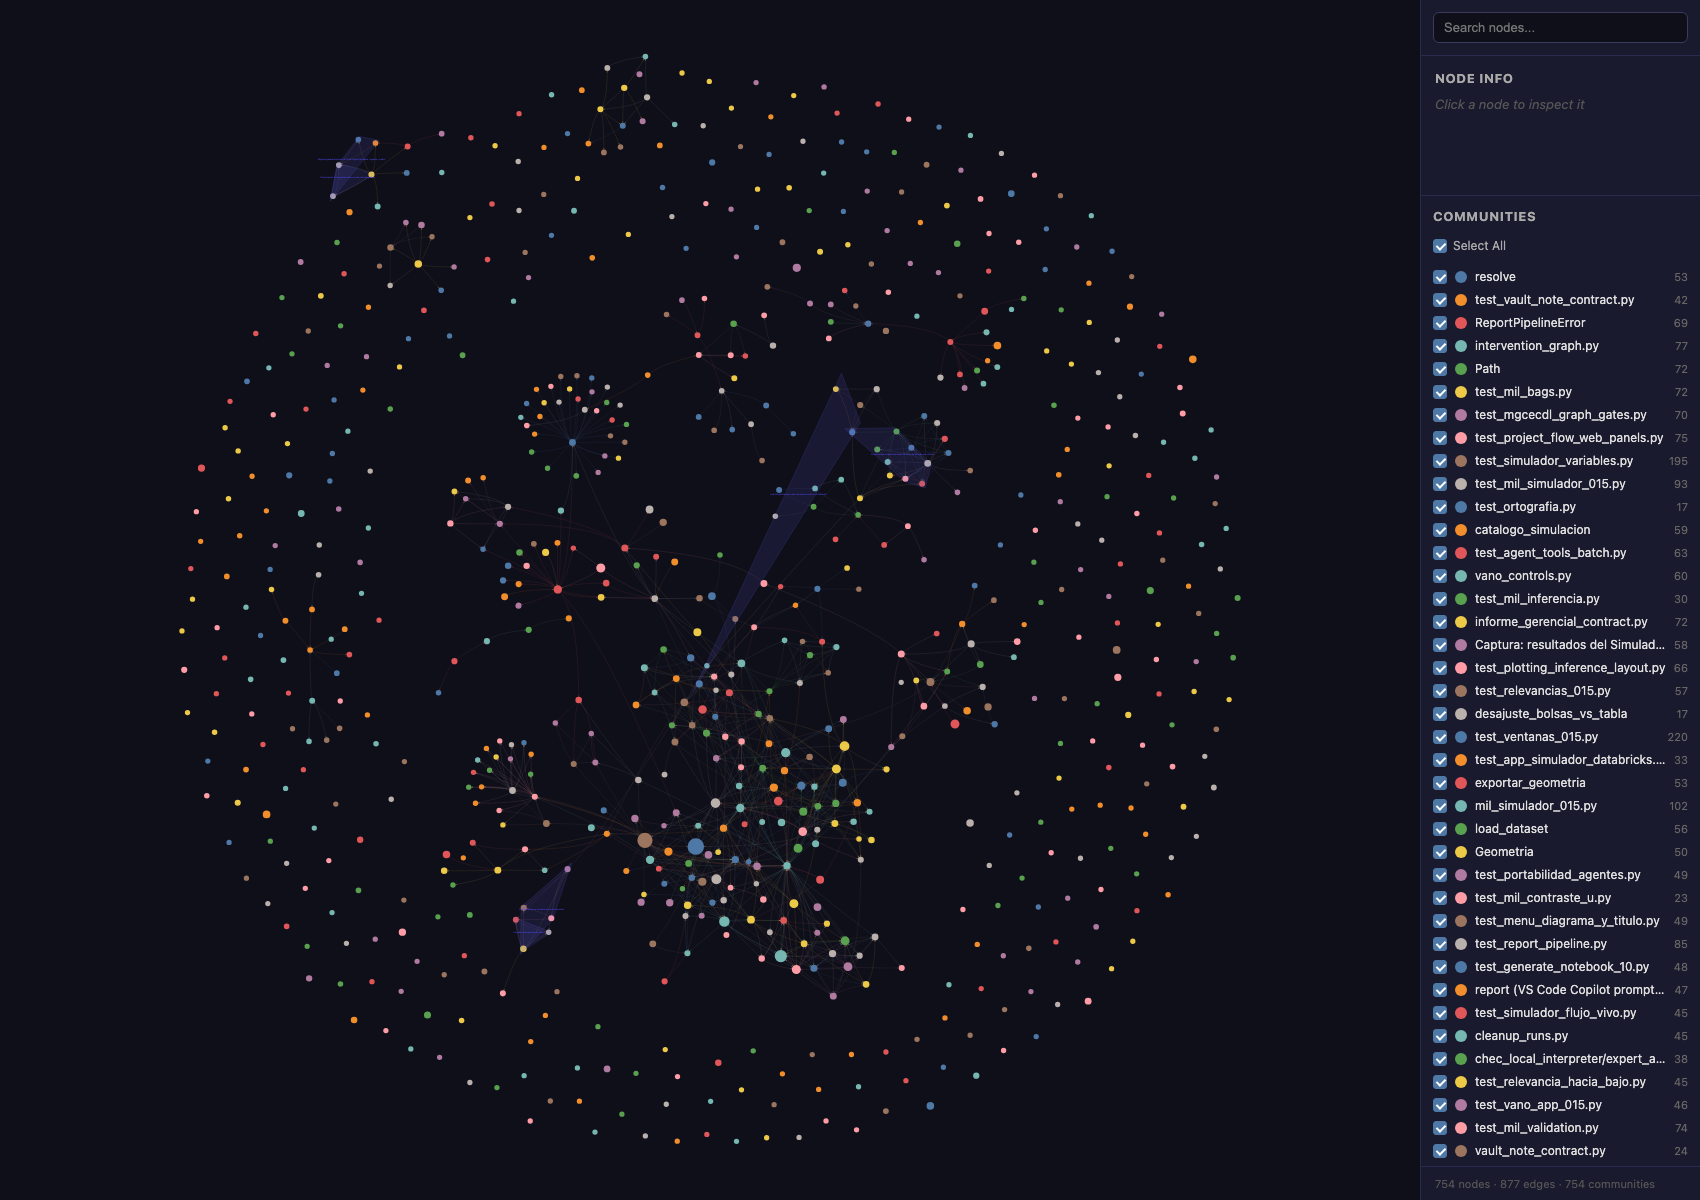
\includegraphics[width=\textwidth]{figures/informe/grafo_proyecto.png}
\caption{Vista agregada del grafo de conocimiento del proyecto: 754 comunidades y las 877
relaciones entre ellas. La visualización es interactiva y permite buscar símbolos por nombre,
seleccionar nodos para consultar su contenido y filtrar comunidades mediante los controles
laterales.}
\label{fig:grafoproyecto}
\end{figure}

Tres precisiones acompañan esta representación:

\begin{itemize}
  \item \textbf{Agregación por comunidades.} Representar simultáneamente alrededor de diez mil
        nodos reduce de forma significativa la legibilidad en el navegador. La vista agregada
        conserva la estructura de relaciones y la hace navegable.
  \item \textbf{Etiquetado automático.} Las comunidades proceden de un algoritmo y no incluyen
        nombre. El nombre mostrado se asigna posteriormente mediante un proceso automático de
        etiquetado basado en su contenido.
  \item \textbf{Se versiona con el código.} El grafo reside en el repositorio y se versiona con
        Git, de modo que cada reconstrucción queda registrada como un cambio revisable y no
        como un archivo transitorio.
\end{itemize}

Su aplicación práctica es identificar dependencias, consumidores de código y componentes
potencialmente afectados por una modificación. Ese análisis permitió también identificar y
retirar componentes sin consumidores activos, entre ellos los reportados en la
Tabla~\ref{tab:retiros}.

% ============================================== 13. PRUEBAS ===============
\section{Pruebas y validación}
\label{sec:pruebas}

La validación se organiza por tipos de evidencia. El repositorio incorpora una suite de
\textbf{3.278 pruebas automatizadas} repartidas en 182 archivos --- 3.226 se ejecutan y 52 se
omiten por depender de un entorno que no siempre está disponible ---, que cubren la carga de datos,
la construcción de contexto, los contratos de salida de los agentes, la validación de esas
salidas, la alineación experta, la inferencia del modelo, la disposición de las gráficas, las
ventanas y la geometría de criticidad, el simulador por vano, el archivo de simulaciones, el
catálogo de costos, el empaquetado de las aplicaciones y el contrato del despliegue a
Databricks.

Se contemplan además evaluaciones fuera de línea con contextos sintéticos, que verifican que las
instrucciones y las respuestas respeten los contratos, la estructura JSON, las variables
permitidas, el manejo de datos faltantes y la separación entre explicación histórica, inferencia
predictiva y comparación experta.

El protocolo de validación del modelo por bolsas y su resultado se detallan en la
Sección~\ref{sec:validacion}: veredicto no alcanzado, con la brecha frente a la línea base por
debajo del ruido de entrenamiento medido.

La publicación web cuenta con flujo de construcción propio y despliegue automático, lo que
permite someter resultados a revisión técnica sin depender de una aplicación de servidor activa.
Los tableros que requieren núcleo de cómputo vivo se publican por separado como aplicaciones
Databricks.

% ============================================== 14. COSTO OPERATIVO =======
\section{Estimación de costo operativo en Azure Databricks}

Esta sección complementa el alcance técnico con un orden de magnitud del costo de operar el
flujo en la nube. Las tarifas de Azure, Databricks y los proveedores de modelo de lenguaje se
incorporaron el 30 de junio de 2026 y deben verificarse contra la tarifa vigente antes de
utilizarse para planeación. La estimación asume \textbf{una ejecución completa del flujo ya
estabilizado}: no incluye iteraciones para afinar la migración, depurar errores, ajustar rutas,
instalar dependencias, repetir cuadernos, validar credenciales ni probar configuraciones de
clúster.

Se emplean dos siglas propias de la plataforma. DBU (\emph{Databricks Unit}) es la unidad de
consumo con la que Databricks factura el procesamiento, adicional al costo de las máquinas
virtuales. FMS (\emph{Foundation Model Serving}) es el servicio administrado de Databricks para
consultar modelos fundacionales sin desplegarlos por cuenta propia.

\begin{table}[H]
\centering
\caption{Comparación de escenarios de operación, por ejecución completa del flujo}
\label{tab:costosdbx}
\small
\begin{tabularx}{\textwidth}{L{3.0cm} X L{3.0cm} r}
\toprule
\textbf{Escenario} & \textbf{Configuración de cómputo} & \textbf{Modelo de lenguaje} & \textbf{Costo aprox.} \\
\midrule
Ajuste interactivo & Clúster interactivo con GPU T4 para todo el flujo & Interfaz externa o FMS & USD 5--8 \\
Ajuste interactivo & Igual, con 30 a 60 min de inactividad & Cualquiera & USD 6--9 \\
Producción & Trabajos programados, con CPU y GPU separadas & Interfaz externa o FMS & USD 4--6 \\
Producción degradada & Clúster interactivo con inactividad prolongada o terminación automática inadecuada & Cualquiera & USD 8--15$+$ \\
\midrule
Modelo local 32B$+$ & GPU A100 de 80 GB, por hora & Sin servicio externo & USD 4,5--8/h \\
Modelo local 32B$+$ & La misma, en operación permanente & Sin servicio externo & USD 3.300--5.800/mes \\
\bottomrule
\end{tabularx}
\end{table}

Tres conclusiones se derivan de la comparación. El costo del modelo de lenguaje por interfaz
externa o por FMS resulta bajo frente al costo de GPU y DBU --- por debajo de USD 0,30 por ciclo
base ---, de modo que la elección entre proveedores debe tomarse por gobierno, trazabilidad,
privacidad y política empresarial, y no por costo. Separar CPU y GPU mediante trabajos
programados reduce el costo de la ejecución completa. Y los modelos locales de 32.000 millones de
parámetros o superiores deben tratarse como escenario independiente, porque requieren
aceleradores dedicados y agregan un costo por hora que no se amortiza salvo que exista un
requisito de privacidad o de control del modelo que lo justifique.

\begin{table}[H]
\centering
\caption{Referencia de tiempos de la cadena secuencial con GPU}
\label{tab:tiemposdbx}
\small
\begin{tabularx}{\textwidth}{X r}
\toprule
\textbf{Etapa} & \textbf{Tiempo} \\
\midrule
Enriquecimiento climático & 36,5 min \\
Búsqueda de hiperparámetros (20 ensayos) & 2 h \\
Entrenamiento (100 épocas) & 10 min \\
Evaluación de desempeño & 1 min \\
Análisis por circuito & 5 min \\
Replicación documental & 2 h 30 min \\
\midrule
\textbf{Total aproximado} & \textbf{5,38 h} \\
\bottomrule
\end{tabularx}
\end{table}

\paragraph{Alcance de esta referencia.} Los tiempos de la Tabla~\ref{tab:tiemposdbx}
corresponden a la cadena completa de nueve cuadernos vigente al momento de la estimación, cuyo
componente dominante era la replicación documental. El flujo actual es sustancialmente más
ligero: el entrenamiento del modelo por bolsas se resuelve en unos diez minutos y
\textbf{no requiere GPU} (Tabla~\ref{tab:dispositivo}), y las dos aplicaciones desplegadas no
ejecutan entrenamiento alguno. La estimación se conserva como cota superior de planeación y no
como el costo del despliegue descrito en la Sección~\ref{sec:databricks}.

% ============================================== 15. ENTREGABLES ===========
\section{Entregables y enlaces}

\begin{table}[H]
\centering
\caption{Entregables remotos y evidencias disponibles}
\label{tab:entregables}
\small
\begin{tabularx}{\textwidth}{L{3.1cm} L{4.6cm} X}
\toprule
\textbf{Entregable} & \textbf{Alcance} & \textbf{Enlace} \\
\midrule
Repositorio técnico & Modelo por bolsas, simulador por vano, tableros, agentes, costos, despliegue y publicación web. Incluye la suite de 3.278 pruebas automatizadas. & \url{https://github.com/amalvarezme/chec-local-uiti-vano-interpreter} \\
Sitio público técnico & Publicación con las visualizaciones, la arquitectura, el modelo, los agentes y los resultados interactivos. & \url{https://amalvarezme.github.io/chec-local-uiti-vano-interpreter/} \\
Sitio base del proyecto & Página institucional del proyecto CHEC--UNAL. & \url{https://amalvarezme.github.io/CHECUNAL_2026/} \\
Repositorio del tablero & Código del tablero Dash, servicios y ruta de paridad reportada previamente. & \url{https://github.com/amalvarezme/dashboard_chec} \\
\bottomrule
\end{tabularx}
\end{table}

% ===================================================== 16. CONCLUSIONES ====
\section{Conclusiones}

El desarrollo consolidó el paso del diagnóstico a la simulación. El sistema ya no se limita a
explicar el comportamiento histórico de \texttt{UITI\_VANO}: responde, para un vano y una ventana
concretos, qué variable modificar y hasta qué valor para que descienda de grupo de criticidad,
entrega esa respuesta en un tablero interactivo con su costo cotizado sobre el catálogo del
contrato, y permite archivar y recuperar cada ejecución. La unidad de análisis quedó alineada con
la unidad de decisión, que es el activo sobre el cual se emite una orden de trabajo.

La incorporación del grafo de restricciones físicas como término de la función de costo, y no
como validación posterior, mantiene la explicación dentro de las relaciones que el personal
técnico reconoce. La medición asociada indica, sin embargo, que con los pesos actuales ese
término apenas participa del gradiente, de modo que su aporte real debe establecerse mediante una
ablación explícita antes de atribuirle efecto.

El protocolo de validación del modelo no alcanzó la barra preregistrada. El análisis del
resultado muestra que la brecha frente a la mejor línea base es menor que el ruido de
entrenamiento observado, por lo que la prioridad técnica inmediata es estabilizar el determinismo
del entrenamiento antes de comparar variantes o continuar la búsqueda de hiperparámetros. El
perfil de error resulta, no obstante, adecuado para priorización operativa: el mejor desempeño se
obtiene sobre la clase Alto y la confusión se concentra en clases contiguas.

Tres decisiones sostienen la trazabilidad del conjunto y conviene mantenerlas: la geometría de
criticidad se congela y se verifica por firma, de modo que el mapa observado y el simulado son
comparables por construcción; el efecto simulado y el costo cotizado permanecen desacoplados,
porque unirlos sin respaldo produciría una cifra con apariencia de estimación de beneficio; y el
razonamiento en lenguaje natural queda fuera del código Python, sujeto a contratos de salida que
se validan antes de publicar.

La combinación de estos elementos con la copia reproducible del dominio en Databricks y con la
instalación asistida constituye una base verificable para la priorización de intervenciones y la
generación de reportes de evidencia.

\vspace{22mm}

\begin{flushright}
\begin{minipage}{9.5cm}
\raggedleft
\rule{7cm}{0.4pt}\\[2pt]
Dir. Proyecto UNAL\\
Prof. Andrés Marino Álvarez Meza\\
\footnotesize Departamento de Ingeniería Eléctrica, Electrónica y Computación\\
Universidad Nacional de Colombia Sede Manizales
\end{minipage}
\end{flushright}

\end{document}
